% Options for packages loaded elsewhere
\PassOptionsToPackage{unicode}{hyperref}
\PassOptionsToPackage{hyphens}{url}
\PassOptionsToPackage{dvipsnames,svgnames,x11names}{xcolor}
%
\documentclass[
  letterpaper,
  DIV=11,
  numbers=noendperiod]{scrartcl}

\usepackage{amsmath,amssymb}
\usepackage{iftex}
\ifPDFTeX
  \usepackage[T1]{fontenc}
  \usepackage[utf8]{inputenc}
  \usepackage{textcomp} % provide euro and other symbols
\else % if luatex or xetex
  \usepackage{unicode-math}
  \defaultfontfeatures{Scale=MatchLowercase}
  \defaultfontfeatures[\rmfamily]{Ligatures=TeX,Scale=1}
\fi
\usepackage{lmodern}
\ifPDFTeX\else  
    % xetex/luatex font selection
\fi
% Use upquote if available, for straight quotes in verbatim environments
\IfFileExists{upquote.sty}{\usepackage{upquote}}{}
\IfFileExists{microtype.sty}{% use microtype if available
  \usepackage[]{microtype}
  \UseMicrotypeSet[protrusion]{basicmath} % disable protrusion for tt fonts
}{}
\makeatletter
\@ifundefined{KOMAClassName}{% if non-KOMA class
  \IfFileExists{parskip.sty}{%
    \usepackage{parskip}
  }{% else
    \setlength{\parindent}{0pt}
    \setlength{\parskip}{6pt plus 2pt minus 1pt}}
}{% if KOMA class
  \KOMAoptions{parskip=half}}
\makeatother
\usepackage{xcolor}
\setlength{\emergencystretch}{3em} % prevent overfull lines
\setcounter{secnumdepth}{5}
% Make \paragraph and \subparagraph free-standing
\ifx\paragraph\undefined\else
  \let\oldparagraph\paragraph
  \renewcommand{\paragraph}[1]{\oldparagraph{#1}\mbox{}}
\fi
\ifx\subparagraph\undefined\else
  \let\oldsubparagraph\subparagraph
  \renewcommand{\subparagraph}[1]{\oldsubparagraph{#1}\mbox{}}
\fi

\usepackage{color}
\usepackage{fancyvrb}
\newcommand{\VerbBar}{|}
\newcommand{\VERB}{\Verb[commandchars=\\\{\}]}
\DefineVerbatimEnvironment{Highlighting}{Verbatim}{commandchars=\\\{\}}
% Add ',fontsize=\small' for more characters per line
\usepackage{framed}
\definecolor{shadecolor}{RGB}{241,243,245}
\newenvironment{Shaded}{\begin{snugshade}}{\end{snugshade}}
\newcommand{\AlertTok}[1]{\textcolor[rgb]{0.68,0.00,0.00}{#1}}
\newcommand{\AnnotationTok}[1]{\textcolor[rgb]{0.37,0.37,0.37}{#1}}
\newcommand{\AttributeTok}[1]{\textcolor[rgb]{0.40,0.45,0.13}{#1}}
\newcommand{\BaseNTok}[1]{\textcolor[rgb]{0.68,0.00,0.00}{#1}}
\newcommand{\BuiltInTok}[1]{\textcolor[rgb]{0.00,0.23,0.31}{#1}}
\newcommand{\CharTok}[1]{\textcolor[rgb]{0.13,0.47,0.30}{#1}}
\newcommand{\CommentTok}[1]{\textcolor[rgb]{0.37,0.37,0.37}{#1}}
\newcommand{\CommentVarTok}[1]{\textcolor[rgb]{0.37,0.37,0.37}{\textit{#1}}}
\newcommand{\ConstantTok}[1]{\textcolor[rgb]{0.56,0.35,0.01}{#1}}
\newcommand{\ControlFlowTok}[1]{\textcolor[rgb]{0.00,0.23,0.31}{#1}}
\newcommand{\DataTypeTok}[1]{\textcolor[rgb]{0.68,0.00,0.00}{#1}}
\newcommand{\DecValTok}[1]{\textcolor[rgb]{0.68,0.00,0.00}{#1}}
\newcommand{\DocumentationTok}[1]{\textcolor[rgb]{0.37,0.37,0.37}{\textit{#1}}}
\newcommand{\ErrorTok}[1]{\textcolor[rgb]{0.68,0.00,0.00}{#1}}
\newcommand{\ExtensionTok}[1]{\textcolor[rgb]{0.00,0.23,0.31}{#1}}
\newcommand{\FloatTok}[1]{\textcolor[rgb]{0.68,0.00,0.00}{#1}}
\newcommand{\FunctionTok}[1]{\textcolor[rgb]{0.28,0.35,0.67}{#1}}
\newcommand{\ImportTok}[1]{\textcolor[rgb]{0.00,0.46,0.62}{#1}}
\newcommand{\InformationTok}[1]{\textcolor[rgb]{0.37,0.37,0.37}{#1}}
\newcommand{\KeywordTok}[1]{\textcolor[rgb]{0.00,0.23,0.31}{#1}}
\newcommand{\NormalTok}[1]{\textcolor[rgb]{0.00,0.23,0.31}{#1}}
\newcommand{\OperatorTok}[1]{\textcolor[rgb]{0.37,0.37,0.37}{#1}}
\newcommand{\OtherTok}[1]{\textcolor[rgb]{0.00,0.23,0.31}{#1}}
\newcommand{\PreprocessorTok}[1]{\textcolor[rgb]{0.68,0.00,0.00}{#1}}
\newcommand{\RegionMarkerTok}[1]{\textcolor[rgb]{0.00,0.23,0.31}{#1}}
\newcommand{\SpecialCharTok}[1]{\textcolor[rgb]{0.37,0.37,0.37}{#1}}
\newcommand{\SpecialStringTok}[1]{\textcolor[rgb]{0.13,0.47,0.30}{#1}}
\newcommand{\StringTok}[1]{\textcolor[rgb]{0.13,0.47,0.30}{#1}}
\newcommand{\VariableTok}[1]{\textcolor[rgb]{0.07,0.07,0.07}{#1}}
\newcommand{\VerbatimStringTok}[1]{\textcolor[rgb]{0.13,0.47,0.30}{#1}}
\newcommand{\WarningTok}[1]{\textcolor[rgb]{0.37,0.37,0.37}{\textit{#1}}}

\providecommand{\tightlist}{%
  \setlength{\itemsep}{0pt}\setlength{\parskip}{0pt}}\usepackage{longtable,booktabs,array}
\usepackage{calc} % for calculating minipage widths
% Correct order of tables after \paragraph or \subparagraph
\usepackage{etoolbox}
\makeatletter
\patchcmd\longtable{\par}{\if@noskipsec\mbox{}\fi\par}{}{}
\makeatother
% Allow footnotes in longtable head/foot
\IfFileExists{footnotehyper.sty}{\usepackage{footnotehyper}}{\usepackage{footnote}}
\makesavenoteenv{longtable}
\usepackage{graphicx}
\makeatletter
\def\maxwidth{\ifdim\Gin@nat@width>\linewidth\linewidth\else\Gin@nat@width\fi}
\def\maxheight{\ifdim\Gin@nat@height>\textheight\textheight\else\Gin@nat@height\fi}
\makeatother
% Scale images if necessary, so that they will not overflow the page
% margins by default, and it is still possible to overwrite the defaults
% using explicit options in \includegraphics[width, height, ...]{}
\setkeys{Gin}{width=\maxwidth,height=\maxheight,keepaspectratio}
% Set default figure placement to htbp
\makeatletter
\def\fps@figure{htbp}
\makeatother
% definitions for citeproc citations
\NewDocumentCommand\citeproctext{}{}
\NewDocumentCommand\citeproc{mm}{%
  \begingroup\def\citeproctext{#2}\cite{#1}\endgroup}
\makeatletter
 % allow citations to break across lines
 \let\@cite@ofmt\@firstofone
 % avoid brackets around text for \cite:
 \def\@biblabel#1{}
 \def\@cite#1#2{{#1\if@tempswa , #2\fi}}
\makeatother
\newlength{\cslhangindent}
\setlength{\cslhangindent}{1.5em}
\newlength{\csllabelwidth}
\setlength{\csllabelwidth}{3em}
\newenvironment{CSLReferences}[2] % #1 hanging-indent, #2 entry-spacing
 {\begin{list}{}{%
  \setlength{\itemindent}{0pt}
  \setlength{\leftmargin}{0pt}
  \setlength{\parsep}{0pt}
  % turn on hanging indent if param 1 is 1
  \ifodd #1
   \setlength{\leftmargin}{\cslhangindent}
   \setlength{\itemindent}{-1\cslhangindent}
  \fi
  % set entry spacing
  \setlength{\itemsep}{#2\baselineskip}}}
 {\end{list}}
\usepackage{calc}
\newcommand{\CSLBlock}[1]{\hfill\break\parbox[t]{\linewidth}{\strut\ignorespaces#1\strut}}
\newcommand{\CSLLeftMargin}[1]{\parbox[t]{\csllabelwidth}{\strut#1\strut}}
\newcommand{\CSLRightInline}[1]{\parbox[t]{\linewidth - \csllabelwidth}{\strut#1\strut}}
\newcommand{\CSLIndent}[1]{\hspace{\cslhangindent}#1}

\KOMAoption{captions}{tableheading}
\makeatletter
\@ifpackageloaded{caption}{}{\usepackage{caption}}
\AtBeginDocument{%
\ifdefined\contentsname
  \renewcommand*\contentsname{Table of contents}
\else
  \newcommand\contentsname{Table of contents}
\fi
\ifdefined\listfigurename
  \renewcommand*\listfigurename{List of Figures}
\else
  \newcommand\listfigurename{List of Figures}
\fi
\ifdefined\listtablename
  \renewcommand*\listtablename{List of Tables}
\else
  \newcommand\listtablename{List of Tables}
\fi
\ifdefined\figurename
  \renewcommand*\figurename{Figure}
\else
  \newcommand\figurename{Figure}
\fi
\ifdefined\tablename
  \renewcommand*\tablename{Table}
\else
  \newcommand\tablename{Table}
\fi
}
\@ifpackageloaded{float}{}{\usepackage{float}}
\floatstyle{ruled}
\@ifundefined{c@chapter}{\newfloat{codelisting}{h}{lop}}{\newfloat{codelisting}{h}{lop}[chapter]}
\floatname{codelisting}{Listing}
\newcommand*\listoflistings{\listof{codelisting}{List of Listings}}
\makeatother
\makeatletter
\makeatother
\makeatletter
\@ifpackageloaded{caption}{}{\usepackage{caption}}
\@ifpackageloaded{subcaption}{}{\usepackage{subcaption}}
\makeatother
\ifLuaTeX
  \usepackage{selnolig}  % disable illegal ligatures
\fi
\usepackage{bookmark}

\IfFileExists{xurl.sty}{\usepackage{xurl}}{} % add URL line breaks if available
\urlstyle{same} % disable monospaced font for URLs
\hypersetup{
  pdftitle={Sample size estimation for task-related functional MRI studies using Bayesian updating},
  pdfauthor={Eduard T. Klapwijk; Joran Jongerling; Herbert Hoijtink; Eveline A. Crone},
  pdfkeywords={power analysis, region of interest, effect size, R
package, sample sizes, Bayesian updating},
  colorlinks=true,
  linkcolor={blue},
  filecolor={Maroon},
  citecolor={Blue},
  urlcolor={Blue},
  pdfcreator={LaTeX via pandoc}}

\title{Sample size estimation for task-related functional MRI studies
using Bayesian updating}
\author{Eduard T. Klapwijk \and Joran Jongerling \and Herbert
Hoijtink \and Eveline A. Crone}
\date{2024-06-21}

\begin{document}
\maketitle
\begin{abstract}
Task-related functional MRI (fMRI) studies need to be properly powered
with an adequate sample size to reliably detect effects of interest. But
for most fMRI studies, it is not straightforward to determine a proper
sample size using power calculations based on published effect sizes.
Here, we present an alternative approach of sample size estimation with
empirical Bayesian updating. First, this method provides an estimate of
the required sample size using existing data from a similar task and
similar region of interest. Using this estimate researchers can plan
their research project, and report empirically determined sample size
estimations in their research proposal or pre-registration. Second,
researchers can expand the sample size estimations with new data. We
illustrate this approach using four existing fMRI data sets where
Cohen's d is the effect size of interest for the hemodynamic response in
the task condition of interest versus a control condition, and where a
Pearson correlation between task effect and age is the covariate of
interest. We show that sample sizes to reliably detect effects differ
between various tasks and regions of interest. We provide an R package
to allow researchers to use Bayesian updating with other task-related
fMRI studies.
\end{abstract}

\section{Introduction}\label{introduction}

Since the emergence of functional magnetic resonance imaging (fMRI),
these techniques have provided unprecedented opportunities to study
functional brain development during childhood and adolescence by
scanning children from the age of four years onward. There is great
progression in the assessment of neural functional growth using
cross-sectional and longitudinal assessments of cognitive, social and
affective processes across the full range of childhood to adulthood.
Despite the advancements in the ability to study the developing brain in
vivo using fMRI, recent years have seen an increased concern about the
replicability of scientific findings in general and particularly in
psychology and cognitive neuroscience (Bishop 2019; E. T. Klapwijk et
al. 2021; Munafò et al. 2017; Poldrack et al. 2017; see Marek et al.
2022 for a similar concern for resting-state functional connectivity and
structural MRI data sets).

Low statistical power due to small sample sizes is arguably one of the
main reasons for lower than desired replicability of study results.
Statistical power is the probability that a study will reject the null
hypothesis when it is false, that is, when there is a non-zero effect
(e.g., Cohen's d or Pearson's correlation) in the population of
interest. Power is determined by the size of the effect, the alpha level
chosen, and the size of the sample (Cohen 1992). The smaller each of
effect size, alpha level, and sample size are, the lower the power.
Since many psychological phenomena consist of relatively subtle, small
effects (Funder and Ozer 2019; Gignac and Szodorai 2016; Yarkoni 2009),
the main source for increasing power, and over which researchers have a
reasonable degree of control, is the sample size (given limited
flexibility of the alpha level). Despite the need for well-powered
studies to reliably detect effects of interest, empirical reports have
shown that most cognitive neuroscience and fMRI studies are underpowered
due to small sample sizes (Button et al. 2013; Maxwell 2004; Nord et al.
2017; Poldrack et al. 2017; Szucs and Ioannidis 2017; Turner et al.
2018). With developmental populations, sufficiently large sample sizes
might be even harder to establish because of the challenges in
recruitment and testing of young participants (Achterberg and Meulen
2019; E. T. Klapwijk et al. 2021).

Recently, well-coordinated efforts and funding have led to several
large-scale projects that collect developmental task-related fMRI data
with larger sample sizes. These projects have the potential to resolve
the problem of power with sample sizes in the thousands, such as the
IMAGEN study (\(N ≈ 2,000\)) (Schumann et al. 2010), the Philadelphia
Neurodevelopmental Cohort (\(N ≈ 1,000\)) (Satterthwaite et al. 2016),
the Human Connectome Project in Development (HCP-D; \(N ≈ 1,300\))
(Somerville et al. 2018), and the Adolescent Brain Cognitive Development
(ABCD) study (\(N ≈ 11,000\)) (Casey et al. 2018). The leap forward made
with this wealth of high-powered, mostly publicly available data can
hardly be overstated, given that they provide an important open research
tool for researchers across the globe.

However, most fMRI studies are carried out by individual research groups
in much smaller samples, which have more opportunities to pursue new
scientific questions, for example using novel paradigms. It is also
vital that the findings of such studies are replicable and meaningful,
meaning that these studies should be properly powered, also without
sample sizes in the range of large multi-lab studies. The main issue
with power analysis is that the effect size in the population of
interest is unknown. One option is to use effect sizes reported in the
literature of the research area at hand. But these effect sizes are
often inflated due to publication bias (Gelman and Carlin 2014;
Ioannidis 2005; Open Science Collaboration 2015; Wicherts et al. 2016;
Yarkoni 2009). Therefore, calculating power based on published effect
sizes usually underestimates the sample size needed to reliably detect
an effect.

This paper will present a novel method to determine the required sample
size for fMRI studies based on existing (i.e., already collected) data
using Bayesian updating (Rouder 2014). Specifically, the approach will
determine the proportion of the already collected data that is needed to
get a desired credible interval (the Bayesian counterpart of the
confidence interval). This will provide an estimate of the percentage of
cases for which the credible interval is expected to be in the desired
range (e.g., the interval should \emph{not} contain the value 0 for the
parameter of interest). This in turn gives us an estimate of the sample
size needed for a certain level of power. The current paper will provide
examples (including an R package) for two effect sizes: Cohen's d and
Pearson's correlation. The sample size determined using existing data is
valuable when designing a new research project and when justifying
sample sizes in a pre-registration or in proposals send to a (medical)
ethical committee.

We will illustrate sample size determination using existing data sets
and tasks that are currently widely used in the developmental fMRI
literature, specifically cognitive control, reward activity, and
social-cognitive processing (see Table~\ref{tbl-1} for an overview)
based on existing data from our own lab. It will be determined how large
the sample size should be to detect Cohen's d, such that 95\% does not
contain the value zero for a specific condition effect (e.g., brain
activity during feedback processing versus rule application). Most prior
developmental fMRI studies addressed the question whether an effect
linearly increases or decreases with age (Crone and Steinbeis 2017). We
therefore also determine the sample size needed to detect a Pearson
correlation of an effect with linear age that is larger than zero. In
the next sections, we will first introduce Bayesian updating, the
highest density credible interval, and sample size determination. Next,
we will provide examples using existing data from four fMRI studies
(Braams et al. 2014; Peters and Crone 2017; Spaans et al. 2023; Cruijsen
et al. 2023), and illustrate sample size determination using these
examples.

\subsection{Bayesian updating}\label{bayesian-updating}

Bayesian updating can be used to determine the sample size required to
estimate Cohen's d or Pearson's correlation with a certain precision.
Precision is presented in the form of a 95\% highest density credible
interval (HDCI), that is, the narrowest possible interval that is
believed to contain the true value of the parameter of interest with a
probability of .95\footnote{In statistical terms: the HDCI contains 95\%
  of the marginal posterior density of the parameter which is a function
  of the information in the data and prior knowledge with respect to the
  parameter.}. The narrower this interval, the higher the precision with
which the parameter is estimated.

Bayesian updating as implemented here relies on the assumption that a
priori, that is, before collecting the data, each possible value of the
parameter of interest is equally likely. This has two implications.
First, the HDCI is completely determined by the data and not by prior
information. Secondly, the numerical values of the estimate and
endpoints of the HDCI are equal to the estimate and endpoints of the
classical confidence interval.

Bayesian updating can be used to determine the smallest sample size for
which the resulting HDCI does not contain the value zero. Bayesian
updating consists of four steps:

\begin{enumerate}
\def\labelenumi{\arabic{enumi}.}
\item
  Determine the maximum achievable size of the sample.
\item
  Collect the data for an initial number of participants and then
  compute the estimate and HDCI. The actual number chosen is irrelevant,
  but with 20 participants the estimate and HDCI will usually give a
  first impression of the size of Cohen's d or Pearson's correlation
  that is not totally determined by sample fluctuations and/or outliers.
\item
  Add several participants to the sample (updating) and recompute the
  estimate and HDCI.
\item
  If the HDCI still contains the value zero and the maximum achievable
  sample size has not been obtained, return to the previous step.
  Otherwise, the updating is finished and estimates and corresponding
  HDCI's are reported.
\end{enumerate}

\subsubsection{The highest density credible interval
(HDCI)}\label{the-highest-density-credible-interval-hdci}

It is important to highlight that the HDCI is not a confidence interval.
If many data sets are sampled from the population of interest and each
data set is used to compute the 95\% confidence interval for the
parameter of interest, then it holds that 95\% of the intervals contain
the true value. However, in contrast to HDCIs, confidence intervals
cannot be updated because their coverage level will become smaller than
95\%. This will be illustrated using a simple example.

Imagine many researchers want to show that Cohen's d is unequal to zero.
Each of them samples a data set with \(n = 20\) for each group from the
population of interest (in which Cohen's d happens to equal zero). About
5\% of the 95\% confidence intervals do not contain the value 0. These
researchers will not continue their efforts; they have ``shown'' that
``their'' effect is not zero. At this stage the Type I error rate is
.05. However, the 95\% remaining researchers increase their power by
updating their data with another 10 persons per group and recompute
their 95\% confidence intervals of which about 2.8\% (number determined
using simulation) does not contain the value 0. Therefore, the Type I
error rate is increased to 5\% + 2.8\% = 7.8\%, that is, the updating
rendered 92.2\% confidence intervals and not 95\% confidence intervals.

A HDCI should therefore not be interpreted in the context of many
hypothetical data sets sampled from the population of interest. The HDCI
is computed using the observed data at hand and is the shortest interval
that is believed to contain the true value of Cohen's d with a
probability of .95. When updating, the size of the data at hand becomes
larger, the information with respect to Cohen's d increases, and
therefore the width of the HDCI becomes smaller. The HDCI summarizes the
evidence in the data at hand with respect to the size of Cohen's d,
which is different from a confidence interval which aims to control
error rates under (hypothetical) repeated sampling from the same
population.

\subsection{Sample Size Determination}\label{sample-size-determination}

The procedure elaborated in this paper is Bayesian (because HDCIs are
used) empirical (because existing data are used) sample size
determination. We use an existing dataset of a certain size, and for all
sample sizes between a minimum (e.g., \(n = 20\)) and maximum sample
size of the sample at hand we compute the HDCI. To account for the
arbitrary order of the participant in a data set, this is done for a set
number of permutations, e.g., 1000, of the participants in the data set.
For each sample size, we then calculate the average HDCI of all
permutations. Considering both the average HDCI and the HDCI's resulting
from the different permutations, will provide an estimate sample size
needed to obtain a 95\% HDCI . The 95\% HDCI for Cohen's d was
established through non-parametric bootstrapping (Efron and Tibshirani
1994). Specifically, we resampled the current subset of data 100 times
and calculated Cohen's d for the difference between variable x and
variable y each time. We then calculated the mean and standard
deviations of Cohen's d across the 100 resampled values. The 95\% CI was
determined by subtracting 1.96 times the standard deviation of the
Cohen's d values from the mean Cohen's d value, and by adding 1.96 times
the standard deviation of the Cohen's d values to the mean Cohen's d
value.

To illustrate the current method, we can take a preview at
Figure~\ref{fig-1} C in the Results section. The dataset used to
construct HDCI's for Cohen's d consists of 149 participants from the
self-evaluation versus control contrast in the medial prefrontal cortex
during a self-evaluation task. In Figure~\ref{fig-1} C the first 20
participants in each of 1000 permuted data sets are used to compute the
HDCI for Cohen's d.~Ten of these intervals are displayed in blue. As can
be seen, of the ten (of 1000) HDCIs displayed, four include the value
zero. Consequently, fluctuations in the order in which participants are
sampled determine whether the HDCI contains the value zero. This is
summarized in Figure~\ref{fig-2} C which shows that the probability that
one of the 1000 HDCIs does not contain the value zero is about 0.6 for
\(n = 20\). In Figure~\ref{fig-1} C, it is shown in the first interval
displayed in purple that the average of the 1000 HDCI's does not contain
the value zero. Therefore, although the average interval does not
contain the value zero, we can learn from the permutations that when
using 20 participants it is still rather likely that the resulting
interval will include the value zero. This becomes much less likely for
the samples of 46 and 72 participants. With these sample sizes neither
the HDCIs nor the average interval contain the value zero (see
Figure~\ref{fig-1} C). Additionally, the probability that an interval
does not contain the value zero equals 100\% for 72 participants (see
Figure~\ref{fig-2} C). Therefore, a sample size of 72 and higher will
usually render intervals that do not contain the value zero.

An issue that sample size determination has in common with power
analysis, is that the effect size in the existing data set will very
likely differ from the effect size in the population that will be
addressed in the study being designed. However, sample size
determination does not suffer from the fact that effect sizes reported
in the literature tend to be inflated (like power analysis) because
effect sizes are straightforwardly computed from actual data. The
determined sample size is therefore an estimate of the required sample
size. This estimate is valuable because it allows researchers to plan
their research project, can be reported in their research proposal or
pre-registration, and it may lead to the conclusion that the sample size
needed cannot be achieved with the resources that you have at your
disposal.

In the next section Bayesian empirical sample size determination will be
exemplified and discussed using different fMRI tasks from the BrainTime
(Braams et al. 2014; Peters and Crone 2017) and Self-Concept (Spaans et
al. 2023; Cruijsen et al. 2023) data sets.

\subsection{\texorpdfstring{\emph{neuroUp} R
package}{neuroUp R package}}\label{neuroup-r-package}

The code for Bayesian updating in this manuscript is implemented in the
R language for statistical computing (R Core Team 2023). We currently
provide the \emph{neuroUp} package at the following location:
\url{https://github.com/eduardklap/neuroUp} (E. Klapwijk, Hoijtink, and
Jongerling 2024). This package is built on several packages from the
tidyverse (Wickham et al. 2019), most notably \emph{ggplot2}. The
package can be installed using the R commands:
\texttt{library(devtools)} and
\texttt{install\_github("eduardklap/neuroUp")}. All data used in the
current manuscript is also available within the \emph{neuroUp} package,
in this way all figures in the manuscript can be reproduced using the R
package. For a more elaborate introduction to \emph{neuroUp} and its
functions, please refer to
\url{https://eduardklap.github.io/neuroUp/articles/neuroUp.html}. To
cite package neuroUp in publications use E. Klapwijk, Hoijtink, and
Jongerling (2024).

\section{Method \& Materials}\label{method-materials}

We focus on sample size estimation for regions of interest from four
different fMRI tasks in two different samples (see Table~\ref{tbl-1}).
We re-used data that has been processed with SPM8 or SPM12 and derived
summary statistics for individual participants for regions and task
conditions of interest (see fMRI processing).

\begin{longtable}[]{@{}
  >{\raggedright\arraybackslash}p{(\columnwidth - 12\tabcolsep) * \real{0.1429}}
  >{\raggedright\arraybackslash}p{(\columnwidth - 12\tabcolsep) * \real{0.1429}}
  >{\raggedright\arraybackslash}p{(\columnwidth - 12\tabcolsep) * \real{0.1429}}
  >{\raggedright\arraybackslash}p{(\columnwidth - 12\tabcolsep) * \real{0.1429}}
  >{\raggedright\arraybackslash}p{(\columnwidth - 12\tabcolsep) * \real{0.1429}}
  >{\raggedright\arraybackslash}p{(\columnwidth - 12\tabcolsep) * \real{0.1429}}
  >{\raggedright\arraybackslash}p{(\columnwidth - 12\tabcolsep) * \real{0.1429}}@{}}
\caption{Overview of tasks processed in the current
study.}\label{tbl-1}\tabularnewline
\toprule\noalign{}
\begin{minipage}[b]{\linewidth}\raggedright
task
\end{minipage} & \begin{minipage}[b]{\linewidth}\raggedright
source
\end{minipage} & \begin{minipage}[b]{\linewidth}\raggedright
associated papers
\end{minipage} & \begin{minipage}[b]{\linewidth}\raggedright
N
\end{minipage} & \begin{minipage}[b]{\linewidth}\raggedright
age range
\end{minipage} & \begin{minipage}[b]{\linewidth}\raggedright
cognitive process
\end{minipage} & \begin{minipage}[b]{\linewidth}\raggedright
region of interest
\end{minipage} \\
\midrule\noalign{}
\endfirsthead
\toprule\noalign{}
\begin{minipage}[b]{\linewidth}\raggedright
task
\end{minipage} & \begin{minipage}[b]{\linewidth}\raggedright
source
\end{minipage} & \begin{minipage}[b]{\linewidth}\raggedright
associated papers
\end{minipage} & \begin{minipage}[b]{\linewidth}\raggedright
N
\end{minipage} & \begin{minipage}[b]{\linewidth}\raggedright
age range
\end{minipage} & \begin{minipage}[b]{\linewidth}\raggedright
cognitive process
\end{minipage} & \begin{minipage}[b]{\linewidth}\raggedright
region of interest
\end{minipage} \\
\midrule\noalign{}
\endhead
\bottomrule\noalign{}
\endlastfoot
Feedback & BrainTime study, Leiden University & (Peters and Crone 2017;
Crone, Duijvenvoorde, and Peper 2016) & 271 & 8-25 yrs & feedback
learning & DLPFC \\
Gambling & BrainTime study, Leiden University & (Braams et al. 2014;
Crone, Duijvenvoorde, and Peper 2016) & 221 & 12-28 yrs &
reward-processing & NAcc \\
Self-evaluations & Self-Concept study, Leiden University & (Cruijsen et
al. 2023; Crone et al. 2022) & 149 & 11-21 yrs & self processing &
mPFC \\
Vicarious charity & Self-Concept study, Leiden University & (Spaans et
al. 2023; Crone et al. 2022) & 156 & 11-21 yrs & vicarious rewards &
NAcc \\
\end{longtable}

\subsection{Data and processing}\label{data-and-processing}

\subsubsection{BrainTime study}\label{braintime-study}

The BrainTime study is an accelerated longitudinal research project of
normative development. A total of 299 participants between ages 8 and 25
years took part in MRI scanning at the first time point. At the second
time point approximately 2 years later, 254 participants were scanned
(most dropout was due to braces, \(n = 33\)). At time point 3,
approximately 2 years after time point 2, 243 participants were scanned
(dropout due to braces: \(n = 11\)). The same Philips 3T MRI scanner and
settings were used for all time points. The following settings were
used: TR = \(2200 ms\), TE = \(30 ms\), sequential acquisition, 38
slices, slice thickness = \(2.75 mm\), field of view (FOV) =
\(220 × 220 × 114.68 mm\). A high-resolution 3D T1 anatomical scan was
acquired (TR = \(9.76 ms\), TE = \(4.59 ms\), 140 slices, voxel size =
\(0.875 × 0.875 × 1.2 mm\), FOV = \(224 × 177 × 168 mm\)).

\paragraph{Feedback task}\label{feedback-task}

For the feedback task (Peters et al. 2014) we included 271 participants
at time point 1 from which region of interest data was available. We use
the same data and processing as reported in (Peters and Crone 2017).
During the task, on each trial participants viewed three squares with a
stimulus presented underneath. Participants were instructed to use
performance feedback to determine which stimulus belonged to which
square. After each choice, feedback was presented to the participant: a
minus sign for negative feedback or a plus sign for positive feedback.
After 12 trials, or when a criterion was reached (placing each of the
three stimuli in the correct box at least two times), a new sequence
with three new stimuli was presented. This criterion was used to strike
a balance between the number of trials in the learning and the
application phase. There were 15 sequences in total, resulting in a
maximum of \(15 x 12 = 180\) trials per participant. For the current
study, we focused on the learning \textgreater{} application contrast,
which compares feedback early in the learning process with feedback for
associations that were already learned (i.e.~application phase).
Individual trial-by-trial analyses were used to determine the learning
and application phase (see Peters and Crone (2017) for details).

\paragraph{Gambling task}\label{gambling-task}

For the Gambling task (Braams et al. 2014), we used data from 221
participant at time point 3 (we went for the largest sample size and
this was the time point with the most data available for the contrasts
of interest). We use the same data and processing as reported in
Schreuders et al. (2018). In the Gambling task, participants could
choose heads or tails and win money when the computer selected the
chosen side of the coin or lose money when the opposite side was
selected. Chances of winning were 50\%. To keep participants engaged,
the number of coins that could be won or lost on varied across trials.
Participants were explained that the coins won in the task would
translate to real money, to be paid out at the end of the experiment.
Gambling was performed in two different conditions: participants played
23 trials for themselves, and 22 trials for their best friend. For the
current study, we focused on reward processing by analysing the winning
for self \textgreater{} losing for self contrast.

\subsubsection{Self-Concept study}\label{self-concept-study}

The Self-Concept study is a cohort-sequential longitudinal study in
which 160 adolescents from 11 to 21 years old took part at the first
time point (see \url{https://osf.io/h7u46} for study overview). MRI
scans were acquired on a Philips 3T MRI scanner with the following
settings: TR = \(2200 ms\), TE = \(30 ms\), sequential acquisition, 37
slices, slice thickness = \(2.75 mm\), FOV = \(220 × 220 × 111.65 mm\).
A high-resolution 3D T1 anatomical scan was acquired (TR = \(9.8 ms\),
TE = \(4.6 ms\), 140 slices, voxel size = \(0.875 × 0.875 × 1.2 mm\),
FOV = \(224 × 178.5 × 168 mm\)).

\paragraph{Self-evaluations task}\label{self-evaluations-task}

For the Self-evaluation task we used the same data and processing as
reported in Cruijsen et al. (2023). In this task, participants read 60
short sentences describing positive or negative traits in the academic,
physical, or prosocial domain (20 per domain; 10 with a positive valence
and 10 with a negative valence). Here we focus on the direct
self-evaluation condition, in which participants had to indicate to what
extent the trait sentences applied to them on a scale of 1 (`not at
all') to 4 (`completely'). In the control condition, participants had to
categorize 20 other trait sentences according to four categories: (1)
school, (2) social, (3) appearance, or (4) I don't know. For the current
study, we focused on the direct self-evaluation versus control contrast.
Eleven participants were excluded due to excessive motion during
scanning (\(\>3 mm, n = 8\)), not completing the scan (\(n = 1\)), and a
technical error (\(n = 2\)), resulting in a total sample of \(N = 149\).

\paragraph{Vicarious Charity task}\label{vicarious-charity-task}

For the Vicarious Charity task, we used the same data and processing as
reported in Spaans et al. (2023). In this task, participants could earn
money for themselves and for a self-chosen charity they selected before
scanning. On every trial, participants could choose one of two curtains
to open. After their button press, the chosen curtain opened to show the
division of the stake between themselves and the charity. The overall
outcome was a division of either €4 or €2 between parties. Unknown to
the participant, every outcome condition occurred 15 times during the
task. Participants were informed beforehand that they received extra
money based on the average of three random outcomes at the end of the
research visit. Here we focus on the self-gain \textgreater{}
both-no-gain contrast. This contrast compares the 30 trials in which
participants gained the full €4 or €2 themselves (i.e., €0 for charity)
against 15 baseline trials in which no money was gained in total (i.e.,
€0 for self and €0 for charity). Two participants were excluded from the
analysis due to excessive movement during scanning (\(>3 mm\)), one due
to signal dropout in the SPM mask including the ventral striatum (this
was assessed by visual inspection of all individual SPM masks), and one
due to a technical error, resulting in a total of \(N = 156\).

\subsubsection{fMRI analysis}\label{fmri-analysis}

FMRI analyses for all four tasks were performed using SPM (Wellcome
Department of Cognitive Neurology, London); SPM8 was used for the
BrainTime data and SPM12 for the Self-Concept data. The following
preprocessing steps were used: slice timing correction, realignment
(motion correction), normalization, and smoothing (6 mm full-width at
half maximum isotropic Gaussian kernel). T1 templates were based on the
MNI305 stereotaxic space. All tasks have an event-related design and
events were time-locked with 0 duration to the moment of feedback
presentation. Six motion regressors were added to the model. All other
trials (i.e., trials that did not result in learning in the Feedback
task or too-late trials) were modeled as events of no interest. These
events were used as covariates in a general linear model together with a
set of cosine functions that high-pass filtered the data. The
least-squares parameter estimates of height of the best-fitting
canonical hemodynamic response function (HRF) for each condition were
used in pair-wise contrasts. The contrast images were submitted to
higher-level group analyses. Region of interest analyses were performed
with the MarsBaR toolbox (Brett et al. 2002).

\paragraph{Regions of interest}\label{regions-of-interest}

For the Feedback task, the atlas-based middle frontal gyrus was used as
a region of interest (Harvard-Oxford cortical atlas; thresholded at
50\%; center-of-mass coordinates \(x = -4, y = 22, z = 43\)). Extracted
parameter estimates for this region were obtained in tabular format from
the authors of Peters and Crone (2017), with one value for the mean
activation during learning and one value for the mean activation during
application for all participants. For the Gambling task, the anatomical
mask of the left nucleus accumbens was used as a region of interest
(Harvard-Oxford subcortical atlas; thresholded at 40\%; 28 voxels
included). Extracted parameter estimates for this region were obtained
in tabular format from the authors of Schreuders et al. (2018), with one
value for the mean activation during winning and one value for the mean
activation during losing for all participants.

For the Self-evaluation task, the region of interest used was a mask of
the left medial prefrontal cortex (\(x = −6, y = 50, z = 4\)) based on a
meta-analysis by Denny et al. (2012). Extracted parameter estimates for
this region were obtained in tabular format from the authors of Cruijsen
et al. (2023), with one value for the mean activation during
self-evaluation and one value for the mean activation during the control
condition for all participants. For the Vicarious Charity task, the
anatomical mask of the left nucleus accumbens was used as a region of
interest (Harvard-Oxford subcortical atlas; thresholded at 40\%;
center-of-mass coordinates \(x = −10, y = 12, z = −7\); 28 voxels
included). Extracted parameter estimates for this region were obtained
in tabular format from the authors of Spaans et al. (2023), with one
value for the mean activation during gaining for self and one value for
the mean activation during no-gain for self and charity for all
participants.

\section{Results}\label{results}

\subsection{Task effects using Cohen's
d}\label{task-effects-using-cohens-d}

The average HDCI was used to determine the optimal sample size for the
four fMRI tasks used. For each task and brain region of interest, we
estimated the sample size required to obtain an average HDCI for Cohen's
d not containing the value zero (Figure~\ref{fig-1} and
Figure~\ref{fig-2}; Table~\ref{tbl-2}). Additionally, we also
established whether it was also the case that a majority of the 1000
underlying HDCIs did not contain the value zero.

In Figure~\ref{fig-1} A, an estimate of the required sample size for
feedback learning processing in the DLPFC (middle frontal gyrus) is
presented. Five groups of HDCI's are presented for sample sizes of 20,
70, 120, 170, and 271 persons, in which 271 is the total group sample
size of the existing data set. As can be seen, already with a sample of
20 participants neither of the 10 permuted HDCIs displayed nor the
average of the 1000 HDCI's contain the value zero. In Figure 2A it can
be seen that the proportion of HDCI's not containing the value zero is
equal to 1.0. This is due to the huge effect size of Cohen's d equal to
about 1.9 (see Table~\ref{tbl-2}). Therefore, already with a sample size
of 20 participants, an effect bigger than zero will be detected for this
task and brain region.

For the task effect of gambling (winning for self \textgreater{} losing
for self contrast) in the NAcc, we can see the results in
Figure~\ref{fig-1} B. Here, with a sample of 20 participants the average
of the 1000 HDCIs does not contain the value zero but some of the 10
HDCI's displayed do. The proportion of HDCI's not containing the value
zero is bigger than 0.8 for 20 participants, but with 60 or more
participants none of the 1000 HDCI's contain zero anymore (Figure 2B).
This is related to the large effect size of Cohen's d equal to about 0.7
(see Table~\ref{tbl-2}). Thus, for this task and brain region, already
with a sample size of 20 participants chances are high that an effect
bigger than zero will be detected. Using sample sizes of 60 or more
participants from this existing data set increases the chances of
detection to 100\%.

In Figure~\ref{fig-1} C, results are plotted for the self-evaluation
task in the mPFC. We see that at a sample size of 20 some of the 10
HDCI's displayed still contain the value 0, but not the average of the
1000 HDCI's. The proportion of HDCI's not containing the value 0 is also
below 1.0, around 0.5, for this task at \(N=20\) (Figure 2C). At the
next step that is plotted for this task (\(n = 46\)), we see that the
proportion of HDCI's not containing the value 0 is only a little below
1.0. Thus, for this task and brain region, at a sample size at 46
participants chances are high that an effect bigger than zero will be
detected.

The results of gaining for self in the NAcc are plotted in
Figure~\ref{fig-1} D. With a sample of 20 participants the average of
the 1000 HDCI's does not contain the value zero but some of the 10
HDCI's displayed do. The proportion of HDCI's not containing the value
zero is around 0.75 (Figure 2D), but at \(n = 47\) the proportion of
HDCI's not containing the value 0 is almost 1.0. Therefore, using 20
participants it is still likely that the resulting interval will include
the value zero. This becomes much less likely for the samples of 47 and
74 persons. With these sample sizes neither the HDCIs nor the average
interval contain the value zero. Additionally, the probability that an
interval does not contain the value zero almost reaches 100\%.
Therefore, for this task and brain region, a sample size of 47 and
higher will usually render intervals that do not contain the value zero.

\begin{figure}[H]

\centering{

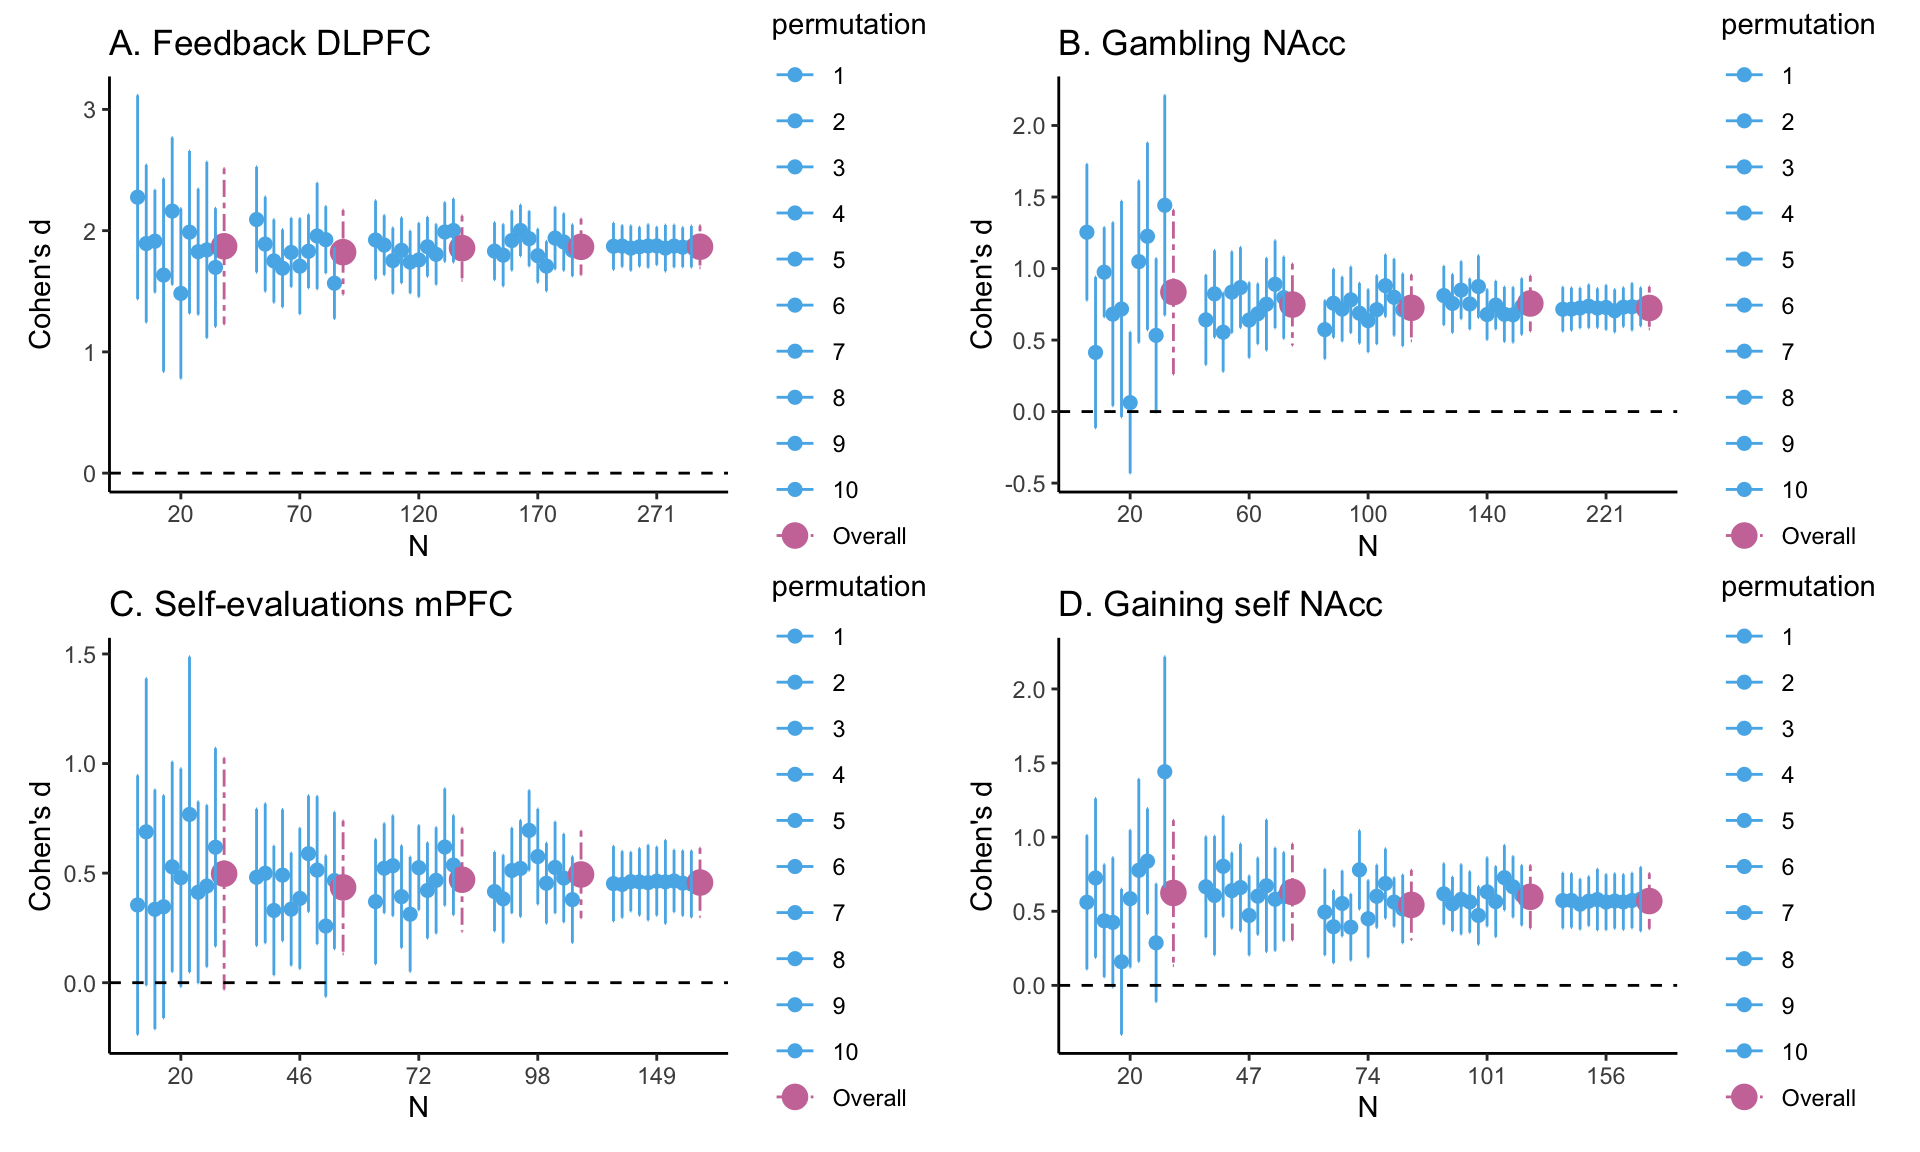
\includegraphics{index_files/figure-latex/figures-cohens_d-fig-1-output-1.png}

}

\caption{\label{fig-1}Estimates of task effects for five different
sample sizes (starting with \(N=20\), then 1/5th parts of the total
dataset). For each sample size 10 randomly chosen HDCI's out of the 1000
HDCI's computed are displayed (in light blue, permutation numbers used
are displayed to the right of each subfigure). The average estimate with
credible interval summarizing the 1000 HDCI's for each sample size are
plotted in reddish purple. DLPFC = dorsolateral prefrontal cortex; mPFC
= medial prefrontal cortex; NAcc = nucleus accumbens.}

\end{figure}%

\textsubscript{Source:
\href{https://eduardklap.github.io/sample-size-test/figures-cohens_d-preview.html\#cell-fig-1}{Code
for Figures 1-2 based on Cohen's d}}

\begin{longtable}[]{@{}
  >{\raggedright\arraybackslash}p{(\columnwidth - 12\tabcolsep) * \real{0.1429}}
  >{\raggedright\arraybackslash}p{(\columnwidth - 12\tabcolsep) * \real{0.1429}}
  >{\raggedright\arraybackslash}p{(\columnwidth - 12\tabcolsep) * \real{0.1429}}
  >{\raggedright\arraybackslash}p{(\columnwidth - 12\tabcolsep) * \real{0.1429}}
  >{\raggedright\arraybackslash}p{(\columnwidth - 12\tabcolsep) * \real{0.1429}}
  >{\raggedright\arraybackslash}p{(\columnwidth - 12\tabcolsep) * \real{0.1429}}
  >{\raggedright\arraybackslash}p{(\columnwidth - 12\tabcolsep) * \real{0.1429}}@{}}
\caption{Mean estimates (with credible interval in brackets) of Cohen's
d for five different sample sizes (starting with n=20, then 1/5th parts
of the total dataset) of the 1000 HDCI's. DLPFC = dorsolateral
prefrontal cortex; mPFC = medial prefrontal cortex; NAcc = nucleus
accumbens.}\label{tbl-2}\tabularnewline
\toprule\noalign{}
\begin{minipage}[b]{\linewidth}\raggedright
\textbf{task}
\end{minipage} & \begin{minipage}[b]{\linewidth}\raggedright
\textbf{brain region}
\end{minipage} & \begin{minipage}[b]{\linewidth}\raggedright
\textbf{n = 20}
\end{minipage} & \begin{minipage}[b]{\linewidth}\raggedright
\textbf{n = 2/5}
\end{minipage} & \begin{minipage}[b]{\linewidth}\raggedright
\textbf{n = 3/5}
\end{minipage} & \begin{minipage}[b]{\linewidth}\raggedright
\textbf{n = 4/5}
\end{minipage} & \begin{minipage}[b]{\linewidth}\raggedright
\textbf{N = total}
\end{minipage} \\
\midrule\noalign{}
\endfirsthead
\toprule\noalign{}
\begin{minipage}[b]{\linewidth}\raggedright
\textbf{task}
\end{minipage} & \begin{minipage}[b]{\linewidth}\raggedright
\textbf{brain region}
\end{minipage} & \begin{minipage}[b]{\linewidth}\raggedright
\textbf{n = 20}
\end{minipage} & \begin{minipage}[b]{\linewidth}\raggedright
\textbf{n = 2/5}
\end{minipage} & \begin{minipage}[b]{\linewidth}\raggedright
\textbf{n = 3/5}
\end{minipage} & \begin{minipage}[b]{\linewidth}\raggedright
\textbf{n = 4/5}
\end{minipage} & \begin{minipage}[b]{\linewidth}\raggedright
\textbf{N = total}
\end{minipage} \\
\midrule\noalign{}
\endhead
\bottomrule\noalign{}
\endlastfoot
Feedback & DLPFC & \textbf{2.03} (1.29, 2.76) & \textbf{1.89} (1.54,
2.25), n = 70 & \textbf{1.88} (1.62, 2.15), n = 120 & \textbf{1.87}
(1.65, 2.1), n = 170 & \textbf{1.87} (1.69, 2.04), \emph{N} = 271 \\
Gambling & NAcc & \textbf{0.8} (0.25, 1.34) & \textbf{0.74} (0.45,
1.03), n = 60 & \textbf{0.73} (0.51, 0.96), n = 100 & \textbf{0.73}
(0.54, 0.92), n = 140 & \textbf{0.73} (0.58, 0.88), \emph{N} = 221 \\
Self-evaluations & mPFC & \textbf{0.5} (0.02, 0.98) & \textbf{0.47}
(0.17, 0.77), n = 46 & \textbf{0.46} (0.22, 0.7), n = 72 & \textbf{0.46}
(0.26, 0.66), n = 98 & \textbf{0.46} (0.29, 0.62), n = 149 \\
Gaining self & NAcc & \textbf{0.64} (0.14, 1.14) & \textbf{0.59} (0.27,
0.91), n = 47 & \textbf{0.58} (0.32, 0.84), n = 74 & \textbf{0.58}
(0.36, 0.8), n = 101 & \textbf{0.57} (0.39, 0.75), \emph{N} = 156 \\
\end{longtable}

\begin{figure}[H]

\centering{

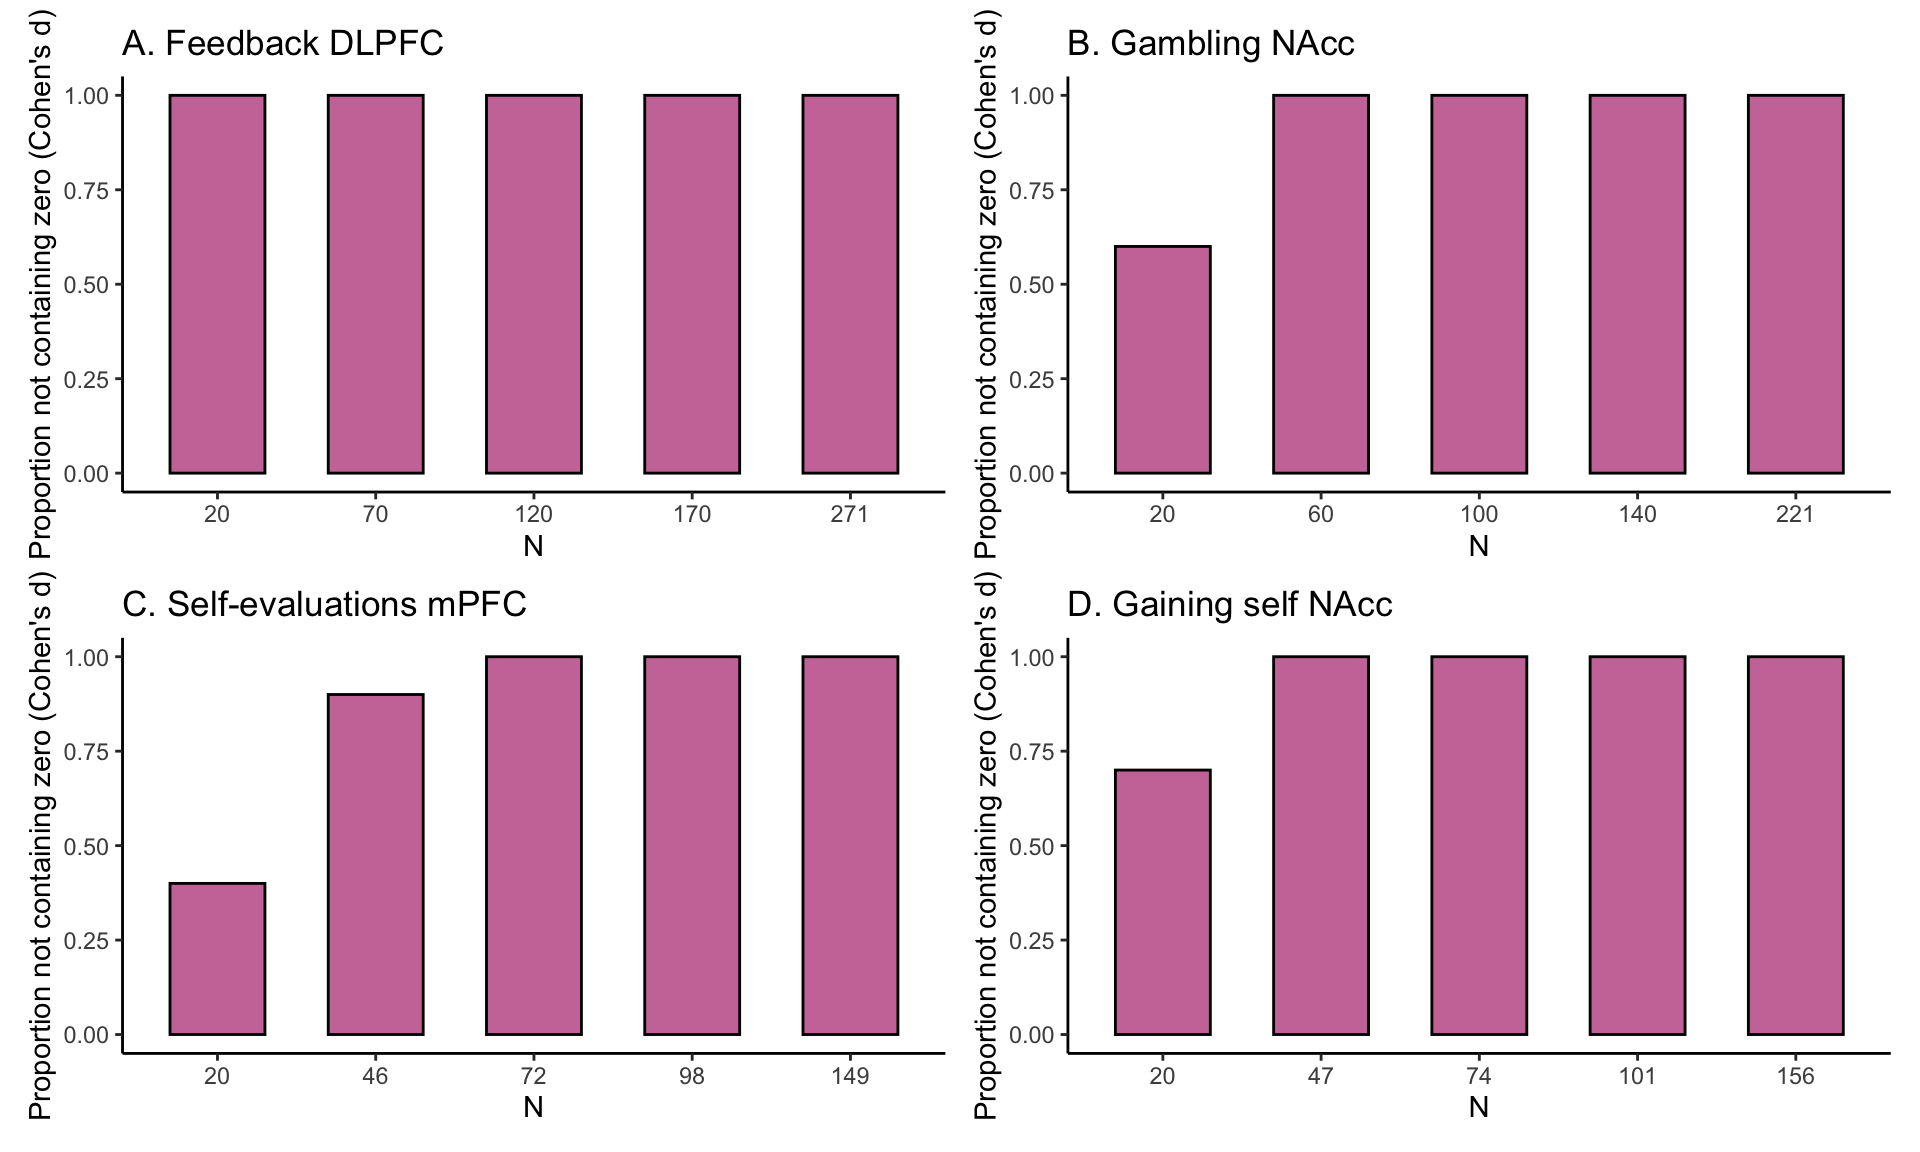
\includegraphics{index_files/figure-latex/figures-cohens_d-fig-2-output-1.png}

}

\caption{\label{fig-2}For each task, for five different sample sizes
(starting with \(n=20\), then 1/5th parts of the total dataset), the
proportion of intervals not containing the value 0 is plotted in reddish
purple.}

\end{figure}%

\textsubscript{Source:
\href{https://eduardklap.github.io/sample-size-test/figures-cohens_d-preview.html\#cell-fig-2}{Code
for Figures 1-2 based on Cohen's d}}

\subsection{Pearson correlations between task effects and
age}\label{pearson-correlations-between-task-effects-and-age}

For each task and brain region of interest we also estimated the sample
size required to obtain an average HDCI for Pearson's correlation
between regional fMRI task responses and age not containing the value
zero (Figure~\ref{fig-3} and Figure~\ref{fig-4}; Table~\ref{tbl-3}) for
which a large proportion of the 1000 HDCI's does not contain the value
zero.

In Figure~\ref{fig-3} A the results are shown for the Pearson's
correlation between age (children and adolescents aged 8-25 years) and
feedback learning processing in the DLPFC. As can be seen, with a sample
of 20 persons the average HDCI contains the value 0. Increasing the
sample size to 70 results in neither of the 10 HDCI's displayed nor the
average of the 1000 HDCI's containing the value 0. We can also see that
the proportion of HDCI's not containing the value zero is less than 0.5
for 20 participants but equal to 1.0 for 70 participants
(Figure~\ref{fig-4} A). Therefore, for a reliable estimate of the
correlation between feedback processing in the DLPFC and age, sample
sizes bigger than 20 are needed.

For the correlation between age and gambling in the NAcc, we can see the
results in Figure~\ref{fig-3} B. Here, for all plotted sample sizes both
the average of the HDCI's and all of the 10 HDCI's displayed do contain
the value zero. The proportion of HDCI's not containing the value zero
is below 0.1 for 20 participants, but with more participants almost all
of the 1000 HDCI's contain the value zero (Figure~\ref{fig-4} B). This
is related to the very small correlation equal to about -0.04 (see
Table~\ref{tbl-3}). Thus, for this task and brain region, it is unlikely
that an effect larger than zero will be detected for a correlation with
age, even with the total sample size of 221 participants.

In Figure~\ref{fig-3} C, results are plotted for the correlation between
age and self-evaluation processing in the mPFC. We see that for all
plotted sample sizes both the average of the 1000 HDCI's and most of the
10 HDCI's displayed do contain the value zero. In Figure~\ref{fig-4} C,
we also see that the proportion of HDCI's not containing the value 0 is
well below 1.0 for all sample sizes shown. Thus, for this task and brain
region, with all available sample sizes the chances are high there will
be no effect detected that is larger than zero. The average Pearson
correlation is also small with a value around 0.13 (Table~\ref{tbl-3}).
The results for the correlation between age and gaining for self in the
NAcc are plotted in Figure 3D. We see that up to 104 participants both
the average of the 1000 HDCI's and most of the 10 HDCI's displayed do
contain the value zero. The proportion of HDCI's not containing the
value zero increases with bigger sample sizes (Figure~\ref{fig-4} A) but
is still below 0.5 for 104 participants. Therefore, with 104
participants it is still likely that the resulting interval will include
the value zero. Therefore, for this task and brain region, with all
available sample sizes the chances are high there will be no effect
detected that is larger than zero. The average Pearson correlation is
also relatively small with a value around -0.18 (Table~\ref{tbl-3}). If
correlations of about -0.18 are considered relevant, the conclusion
might be that one could strive for a sample larger than 160.

\begin{figure}[H]

\centering{

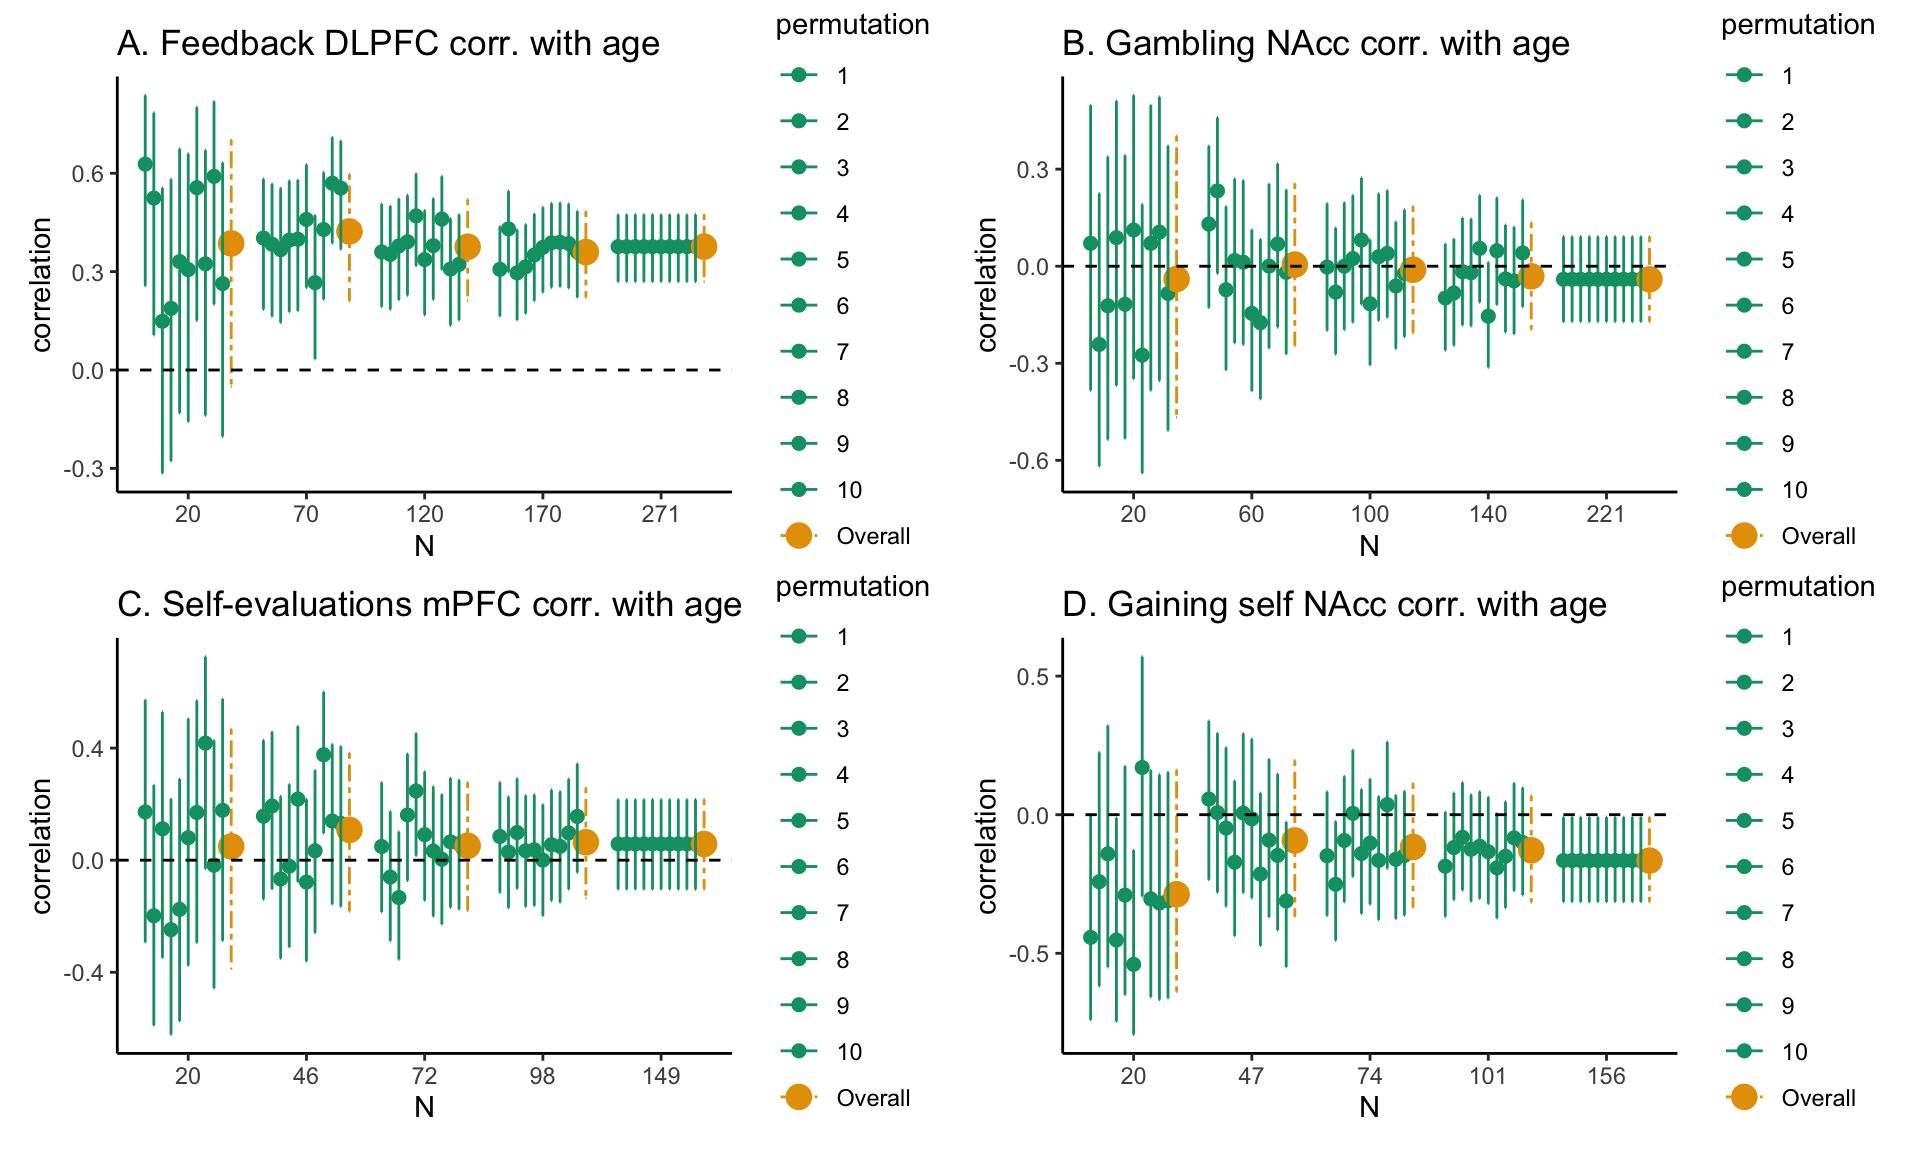
\includegraphics{index_files/figure-latex/figures-correlations-fig-3-output-1.png}

}

\caption{\label{fig-3}Estimates of Pearson's correlation between age and
the task effect for five different sample sizes (starting with \(N=20\),
then 1/5th parts of the total dataset). For each sample size 10 randomly
chosen HDCI's out of the 1000 HDCI's computed are displayed (in green,
permutation numbers used are displayed to the right of each subfigure).
The average estimate with credible interval summarizing the 1000 HDCI's
for each sample size are plotted in orange. DLPFC = dorsolateral
prefrontal cortex; mPFC = medial prefrontal cortex; NAcc = nucleus
accumbens. Age is modeled as linearly increasing or decreasing.}

\end{figure}%

\textsubscript{Source:
\href{https://eduardklap.github.io/sample-size-test/figures-correlations-preview.html\#cell-fig-3}{Code
for Figures 3-4 based on Pearson's correlations}}

\begin{longtable}[]{@{}
  >{\raggedright\arraybackslash}p{(\columnwidth - 12\tabcolsep) * \real{0.1429}}
  >{\raggedright\arraybackslash}p{(\columnwidth - 12\tabcolsep) * \real{0.1429}}
  >{\raggedright\arraybackslash}p{(\columnwidth - 12\tabcolsep) * \real{0.1429}}
  >{\raggedright\arraybackslash}p{(\columnwidth - 12\tabcolsep) * \real{0.1429}}
  >{\raggedright\arraybackslash}p{(\columnwidth - 12\tabcolsep) * \real{0.1429}}
  >{\raggedright\arraybackslash}p{(\columnwidth - 12\tabcolsep) * \real{0.1429}}
  >{\raggedright\arraybackslash}p{(\columnwidth - 12\tabcolsep) * \real{0.1429}}@{}}
\caption{Mean estimates (with credible interval in brackets) of
Pearson's correlation between age and the task effect for five different
sample sizes (starting with N=20, then 1/5th parts of the total dataset)
of the 1000 HDCI's. DLPFC = dorsolateral prefrontal cortex; mPFC =
medial prefrontal cortex; NAcc = nucleus
accumbens.}\label{tbl-3}\tabularnewline
\toprule\noalign{}
\begin{minipage}[b]{\linewidth}\raggedright
task
\end{minipage} & \begin{minipage}[b]{\linewidth}\raggedright
brain region
\end{minipage} & \begin{minipage}[b]{\linewidth}\raggedright
n = 20
\end{minipage} & \begin{minipage}[b]{\linewidth}\raggedright
n = 2/5
\end{minipage} & \begin{minipage}[b]{\linewidth}\raggedright
n = 3/5
\end{minipage} & \begin{minipage}[b]{\linewidth}\raggedright
n = 4/5
\end{minipage} & \begin{minipage}[b]{\linewidth}\raggedright
N = total
\end{minipage} \\
\midrule\noalign{}
\endfirsthead
\toprule\noalign{}
\begin{minipage}[b]{\linewidth}\raggedright
task
\end{minipage} & \begin{minipage}[b]{\linewidth}\raggedright
brain region
\end{minipage} & \begin{minipage}[b]{\linewidth}\raggedright
n = 20
\end{minipage} & \begin{minipage}[b]{\linewidth}\raggedright
n = 2/5
\end{minipage} & \begin{minipage}[b]{\linewidth}\raggedright
n = 3/5
\end{minipage} & \begin{minipage}[b]{\linewidth}\raggedright
n = 4/5
\end{minipage} & \begin{minipage}[b]{\linewidth}\raggedright
N = total
\end{minipage} \\
\midrule\noalign{}
\endhead
\bottomrule\noalign{}
\endlastfoot
Feedback & DLPFC & \textbf{0.38} (-0.06, 0.69 ) & \textbf{0.38} (0.16,
0.56 ), \emph{N} = 70 & \textbf{0.37} (0.21, 0.52 ), \emph{N} = 120 &
\textbf{0.38} (0.24, 0.5 ), \emph{N} = 170 & \textbf{0.38} (0.27, 0.47
), \emph{N} = 271 \\
Gambling & NAcc & \textbf{-0.02} (-0.44, 0.4 ) & \textbf{-0.04} (-0.29,
0.21 ), \emph{N} = 60 & \textbf{-0.04} (-0.23, 0.16 ), \emph{N} = 100 &
\textbf{-0.04} (-0.2, 0.13 ), \emph{N} = 140 & \textbf{-0.04} (-0.17,
0.09 ), \emph{N} = 221 \\
Self-evaluations & mPFC & \textbf{0.07} (-0.36, 0.48 ) & \textbf{0.06}
(-0.23, 0.34 ), \emph{N} = 46 & \textbf{0.06} (-0.17, 0.29 ), \emph{N} =
72 & \textbf{0.06} (-0.14, 0.25 ), \emph{N} = 98 & \textbf{0.06} (-0.1,
0.22 ), \emph{N} = 149 \\
Gaining self & NAcc & \textbf{-0.18} (-0.56, 0.26 ) & \textbf{-0.17}
(-0.44, 0.11 ), \emph{N} = 47 & \textbf{-0.17} (-0.38, 0.06 ), \emph{N}
= 74 & \textbf{-0.17} (-0.35, 0.03 ), \emph{N} = 101 & \textbf{-0.17}
(-0.31, -0.01 ), \emph{N} = 156 \\
\end{longtable}

\begin{Shaded}
\begin{Highlighting}[]
\CommentTok{\# plot figure 4 using patchwork library}
\NormalTok{feedback\_fig$fig\_corr\_nozero }\OperatorTok{+}\NormalTok{ gambling\_fig$fig\_corr\_nozero }\OperatorTok{+}\NormalTok{ selfeval\_fig$fig\_corr\_nozero }\OperatorTok{+}\NormalTok{ vicar\_char\_fig$fig\_corr\_nozero}
\end{Highlighting}
\end{Shaded}

\begin{figure}[H]

\centering{

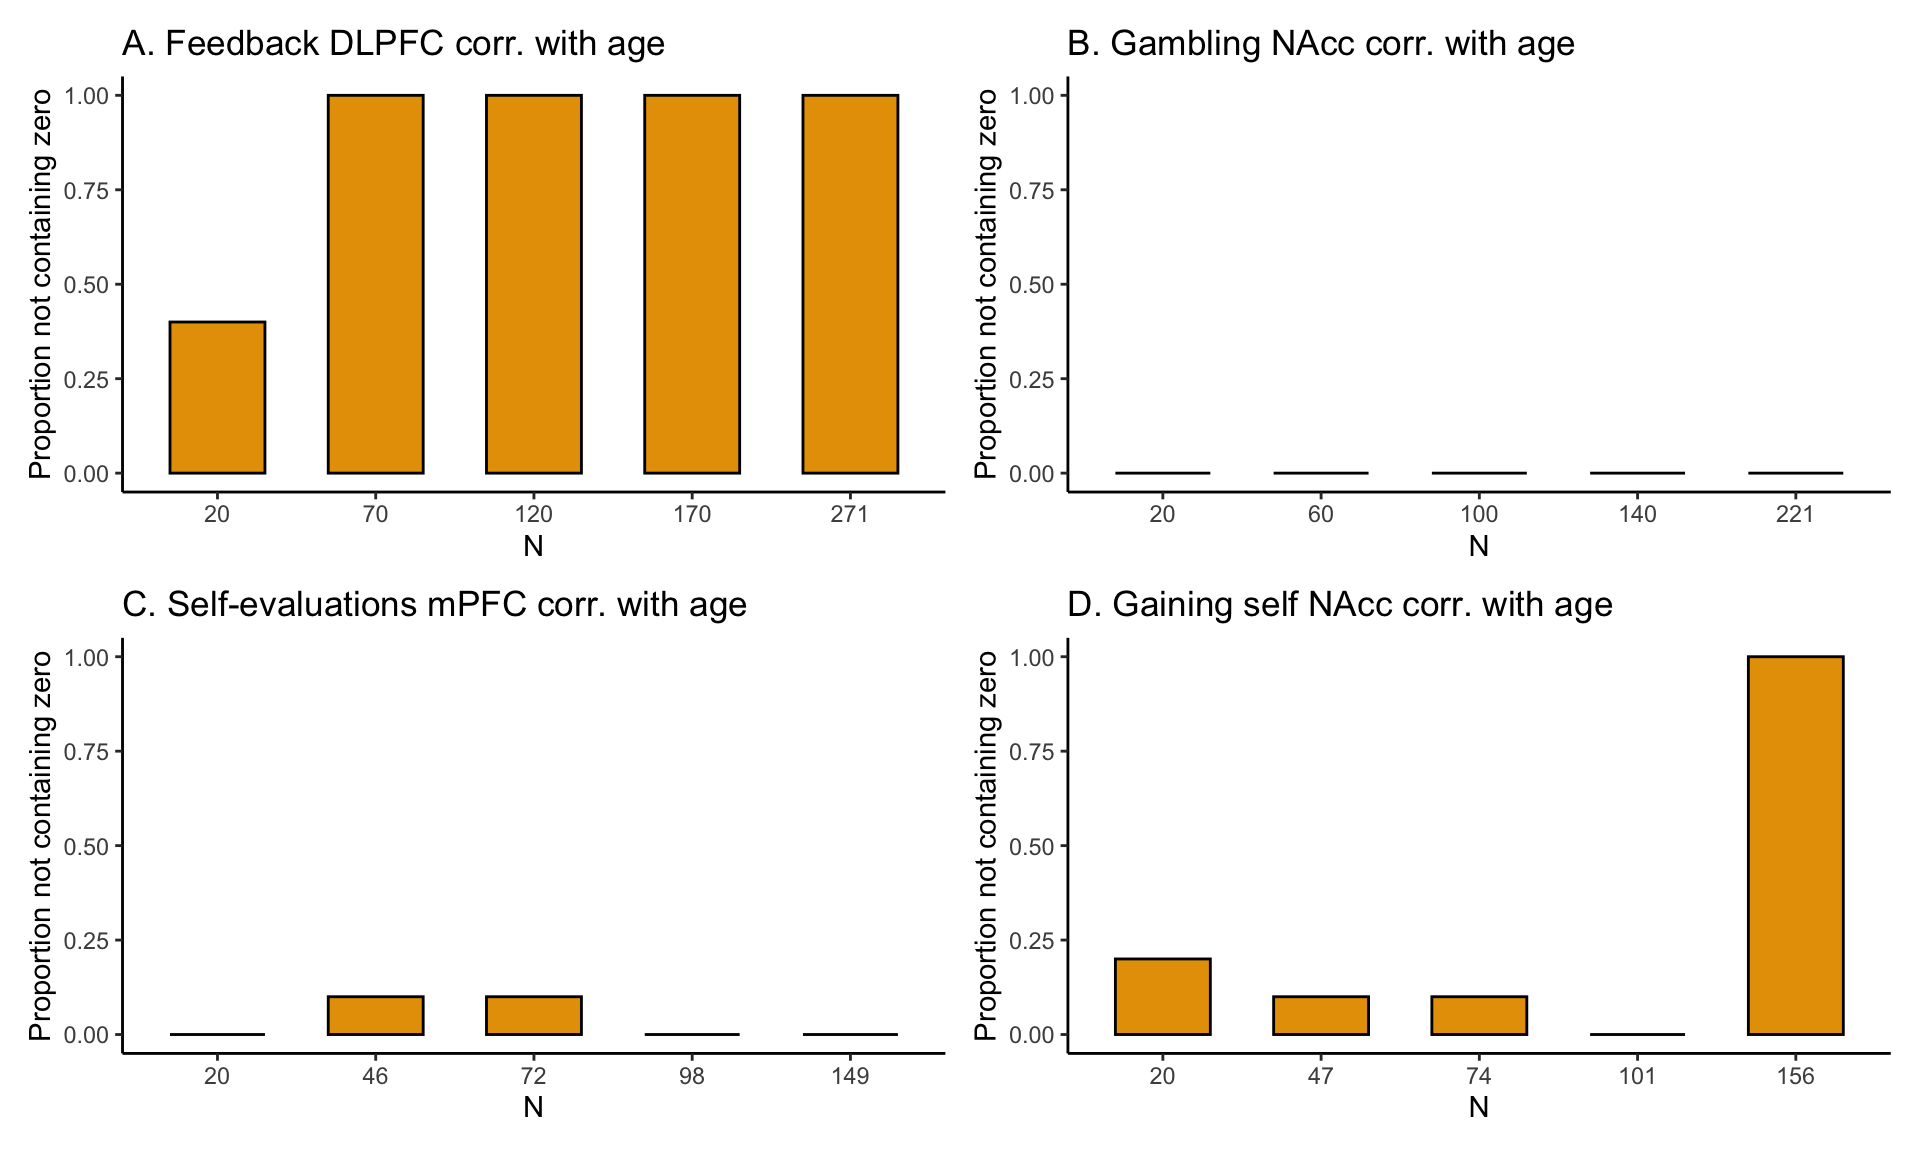
\includegraphics{index_files/figure-latex/figures-correlations-fig-4-output-1.png}

}

\caption{\label{fig-4}For each task, for five different sample sizes
(starting with \(N=20\), then 1/5th parts of the total dataset), the
proportion of intervals not containing the value 0 is plotted in orange.
Age is modeled as linearly increasing or decreasing.}

\end{figure}%

\textsubscript{Source:
\href{https://eduardklap.github.io/sample-size-test/figures-correlations-preview.html\#cell-fig-4}{Code
for Figures 3-4 based on Pearson's correlations}}

\section{Discussion}\label{discussion}

In this paper we tested how existing data can be used to approximately
determine the sample size that is required for a new study that is being
planned. The approach presented has been illustrated using four existing
fMRI studies where Cohen's d is the effect size of interest and four
studies where a Pearson correlation for linear age is of interest.
Additionally, it has been elaborated that Bayesian updating can be used
to deal with the fact that the required sample size can only
approximately be determined. Our results show that calculating and
plotting HDCI's can be helpful in determining at what sample sizes task
effects become more stable. We illustrated with four examples how
researchers can get an indication of the required sample size if they
plan to execute a study that uses feedback learning, reward-processing
(two examples), or self-processing. For all effects under study, the
width of the HDCI became smaller with larger sample sizes, showing that
the precision of the estimation increased with more data. At what sample
size estimations seemed to stabilize for general contrasts (e.g.,
feedback processing versus rule application; reward versus loss)
differed per task and region of interest. For example, the effects in
the middle frontal gyrus during feedback processing were the strongest
of the effects studied here. There, even for sample sizes of 20
participants, task effects clearly differed from zero for the middle
frontal gyrus. But even for such a strong effect, at higher sample sizes
the results became more stable (i.e., less variability in subsamples of
the total dataset). For the other three tasks, the HDCI's still
contained the value zero with 20 participants but at higher sample sizes
of 40-60 participants chances are very high that an effect larger than
zero will be detected. In this paper we tested how existing data can be
used to approximately determine the sample size that is required for a
new study that is being planned. The approach presented has been
illustrated using four existing fMRI studies where Cohen's d is the
effect size of interest and four studies where a Pearson correlation for
linear age is of interest. Additionally, it has been elaborated that
Bayesian updating can be used to deal with the fact that the required
sample size can only approximately be determined.

Our results show that calculating and plotting HDCI's can be helpful in
determining at what sample sizes task effects become more stable. We
illustrated with four examples how researchers can get an indication of
the required sample size if they plan to execute a study that uses
feedback learning, reward-processing (two examples), or self-processing.
For all effects under study, the width of the HDCI became smaller with
larger sample sizes, showing that the precision of the estimation
increased with more data. At what sample size estimations seemed to
stabilize for general contrasts (e.g., feedback processing versus rule
application; reward versus loss) differed per task and region of
interest. For example, the effects in the middle frontal gyrus during
feedback processing were the strongest of the effects studied here.
There, even for sample sizes of 20 participants, task effects clearly
differed from zero for the middle frontal gyrus. But even for such a
strong effect, at higher sample sizes the results became more stable
(i.e., less variability in subsamples of the total dataset). For the
other three tasks, the HDCI's still contained the value zero with 20
participants but at higher sample sizes of 40-60 participants chances
are very high that an effect larger than zero will be detected.

The results are different for the Pearson correlation between linear age
and task effects, as can be seen in Figure~\ref{fig-3} and
Figure~\ref{fig-4}. Here again the results of the middle frontal gyrus
during feedback processing were the strongest. But even for such a
strong effect, the sample size needed to estimate the correlation with
age is much higher than the sample size needed to find a stable task
effect. For the Pearson correlation, only at a sample size of \(N=70\)
or more the lower bound of the credible is above zero, suggesting that
one can be confident that there is a positive Pearson correlation.

For the correlation between linear age (between 12-28 years) and
reward-processing in the NAcc, the results were dependent on the
specific task context. In a gambling task with the contrast reward
versus loss, even with a sample size of 221 the average HDCI contains
the value zero when testing for linear age effects. We found that the
average Pearson correlation is -.04 for this effect, which is so small
that it is likely irrelevant. In contrast, for rewards in a vicarious
reward context with the contrast reward versus no reward, probability of
a positive Pearson correlation with negative age increased with larger
sample sizes and the average CI did just not contain zero using the full
sample size of 156 (\(M = -0.17; 95\% CI [-0.31, -0.01]\)). Note that we
only tested for linear age effects, whereas prior studies reported that
reward processing may be best described by non-linear effects (Braams et
al. 2014); which should be tested in future extensions of the approach
illustrated here. The results described for the linear age effects are
in line with simulation studies suggesting that typically in psychology
relatively large sample sizes of \(N=150\) to \(N=250\) (Schönbrodt and
Perugini 2013) are needed to obtain a study that is sufficiently powered
to evaluate a Pearson correlation with age or psychological variables.

There are different ways in which the methods described here could be
put to practice. When planning to use an existing task for follow-up or
replication research, existing data can be used to provide an educated
guess of the sample size that is needed in the new study (given that the
new samples resemble the existing sample). In this way new task-related
fMRI studies will likely be properly powered, even if these are
small-scale studies from individual labs. Even in the current era of
large-scale consortium studies, there remains the need to conduct
studies with more modest sample sizes. Such studies can help to balance
between methodological robustness of well-established experiments and
experimental design novelty. These data sets could complement large,
public data sets with more idiosyncratic tasks and specific samples.
Furthermore, sample size determination using existing data can be
combined with Bayesian updating when collecting new data for a new
research project. The following steps can be used:

\begin{enumerate}
\def\labelenumi{\arabic{enumi}.}
\item
  Execute Bayesian empirical sample size determination. This will render
  an estimate of the sample size needed for an adequately powered study.
\item
  Execute the planned study with the sample size determined in the
  previous step.
\item
  Compute the effect size of interest (e.g., Cohen's d or Pearson's
  correlation) and the corresponding HDCI.
\item
  Evaluate the HDCI:

  \begin{enumerate}
  \def\labelenumii{\alph{enumii}.}
  \item
    If the HDCI does not contain the value zero, your study is finished.
  \item
    If the HDCI does contain the value zero, there are two options:

    \begin{enumerate}
    \def\labelenumiii{\roman{enumiii}.}
    \item
      If the estimate of the effect size is close to zero, the effect
      size is small. Adding more data (updating) may (or may not) render
      an HDCI that does not contain the value but will very likely still
      render an effect size that is so small that it is irrelevant.
    \item
      If the estimated effect size is relevant in the context of the
      study being executed, it may very well be (but there is no
      certainty) that collecting additional data (updating) will render
      a HDCI that does not contain the value zero. If you have the
      resources, it may be worthwhile to collect additional data and
      return to Step 3). If you do not have the resources, your study is
      finished.
    \end{enumerate}
  \end{enumerate}
\end{enumerate}

In this paper the focus was on Cohen's d and the Pearson correlation,
however, the approach presented can straightforwardly be generalized to
other statistical models and effect size measures. A relatively simple
example is quadratic regression with either Spearman's correlation or
the multiple correlation as the effect size measure, but generalizations
to more involved statistical models are conceivable. Arguably, in more
complex statistical models our approach may succeed where classical
power analysis may very well fail. The reason for the latter is that in
power analysis ``the effect size'' has to be specified. In, for example,
structural equation models, this implies that factor loadings,
regression coefficients and (co)variances have to be specified. Doing
this such that the specification represents a certain ``effect size'' is
at least difficult and maybe even impossible. In our approach effect
sizes do not have to be specified but are straightforwardly estimated
using existing data. The latter is usually easy and straightforward.
Therefore, in an era of open science in which data sets are increasingly
available for re-use (also for sample size determination) there is a lot
of potential for the approach presented in this paper.

\subsubsection{Practical
recommendations}\label{practical-recommendations}

When calculating HDCI's using existing data, we should keep in mind that
the determined sample size is only an indication of the sample size
required for the new study. In the new study the unknown effect size
(Cohen's d or Pearson's correlation) may be smaller or larger than in
the existing study and therefore a somewhat smaller or larger sample
size may be required. As elaborated earlier, this can be accommodated
using Bayesian updating using the determined sample size as the point of
departure. It is also important to consider how one can determine the
resemblance of a ``to be planned study'' to the existing study. Although
this is a subjective evaluation, it is probably wise to be mindful of
different factors that can influence the strength of the effect, such as
task domain, number of trials, region of interest, and modality (e.g.,
visual versus verbal) (Bennett and Miller 2013; Elliott et al. 2020;
Herting et al. 2018). This is also important for cases where the
ultimate consequence of the sample size estimation might be that one
should not execute the planned study. For example, if a study resembles
study B in Figure 3, it is to be expected that the effect size for
linear correlations with age (if one expects a linear and not a
non-linear effect) is so small that either it is irrelevant, or
unrealistic large sample sizes are required to obtain an average HDCI
that does not contain zero. But even in this situation, it depends on
the context whether something is a meaningful small effect or a
negligible small effect (see for further discussions Dick et al. (2021)
and Funder and Ozer (2019)). One might still decide to continue the
study when there is evidence that the effect at hand is meaningful
because cumulatively it can lead to larger effects. If the effect is yet
deemed irrelevant, one could choose not to collect new data, or one
could alternatively take a bet to pilot a novel version of a similar
task might lead to a stronger effect. Bayesian updating can then be used
to estimate the HDCI's again after a small number of participants. If
the average effect is still close to zero it is probably better to abort
the study.

\section{Acknowledgments}\label{acknowledgments}

This study was funded by the NWO Spinoza prize awarded to Eveline A.
Crone. The authors thank Sabine Peters, Lisa Schreuders, Jochem Spaans,
and Renske van der Cruijsen for providing the ROI data files used in the
paper.

\subsection*{References}\label{references}
\addcontentsline{toc}{subsection}{References}

\phantomsection\label{refs}
\begin{CSLReferences}{1}{0}
\bibitem[\citeproctext]{ref-achterberg2019}
Achterberg, Michelle, and Mara van der Meulen. 2019. {``Genetic and
Environmental Influences on MRI Scan Quantity and Quality.''}
\emph{Developmental Cognitive Neuroscience} 38 (August): 100667.
\url{https://doi.org/10.1016/j.dcn.2019.100667}.

\bibitem[\citeproctext]{ref-bennett2013}
Bennett, Craig M., and Michael B. Miller. 2013. {``fMRI Reliability:
Influences of Task and Experimental Design.''} \emph{Cognitive,
Affective, \& Behavioral Neuroscience} 13 (4): 690--702.
\url{https://doi.org/10.3758/s13415-013-0195-1}.

\bibitem[\citeproctext]{ref-bishop2019}
Bishop, Dorothy. 2019. {``Rein in the Four Horsemen of
Irreproducibility.''} \emph{Nature} 568 (7753): 435--35.
\url{https://doi.org/10.1038/d41586-019-01307-2}.

\bibitem[\citeproctext]{ref-braams2014}
Braams, Barbara R., Sabine Peters, Jiska S. Peper, Berna Güroğlu, and
Eveline A. Crone. 2014. {``Gambling for Self, Friends, and Antagonists:
Differential Contributions of Affective and Social Brain Regions on
Adolescent Reward Processing.''} \emph{NeuroImage} 100 (October):
281--89. \url{https://doi.org/10.1016/j.neuroimage.2014.06.020}.

\bibitem[\citeproctext]{ref-brett2002}
Brett, Matthew, Jean-Luc Anton, Romain Valabregue, and Jean-Baptiste
Poline. 2002. {``Region of Interest Analysis Using an SPM Toolbox.''}
\emph{8th International Conference on Functional Mapping of the Human
Brain} 16 (2): 497.

\bibitem[\citeproctext]{ref-button2013}
Button, Katherine S., John P. A. Ioannidis, Claire Mokrysz, Brian A.
Nosek, Jonathan Flint, Emma S. J. Robinson, and Marcus R. Munafò. 2013.
{``Power Failure: Why Small Sample Size Undermines the Reliability of
Neuroscience.''} \emph{Nature Reviews Neuroscience} 14 (5): 365--76.
\url{https://doi.org/10.1038/nrn3475}.

\bibitem[\citeproctext]{ref-casey2018}
Casey, B. J., Tariq Cannonier, May I. Conley, Alexandra O. Cohen, Deanna
M. Barch, Mary M. Heitzeg, Mary E. Soules, et al. 2018. {``The
Adolescent Brain Cognitive Development (ABCD) Study: Imaging Acquisition
Across 21 Sites.''} \emph{Developmental Cognitive Neuroscience}, The
adolescent brain cognitive development (ABCD) consortium: Rationale,
aims, and assessment strategy, 32 (August): 43--54.
\url{https://doi.org/10.1016/j.dcn.2018.03.001}.

\bibitem[\citeproctext]{ref-cohen1992}
Cohen, Jacob. 1992. {``A Power Primer.''} \emph{Psychological Bulletin}
112 (1): 155--59. \url{https://doi.org/10.1037/0033-2909.112.1.155}.

\bibitem[\citeproctext]{ref-crone2016}
Crone, Eveline A., Anna C. K. van Duijvenvoorde, and Jiska S. Peper.
2016. {``Annual Research Review: Neural Contributions to Risk-Taking in
Adolescence {\textendash} Developmental Changes and Individual
Differences.''} \emph{Journal of Child Psychology and Psychiatry} 57
(3): 353--68. \url{https://doi.org/10.1111/jcpp.12502}.

\bibitem[\citeproctext]{ref-crone2022}
Crone, Eveline A., Kayla H. Green, Ilse H. van de Groep, and Renske van
der Cruijsen. 2022. {``A Neurocognitive Model of Self-Concept
Development in Adolescence.''} \emph{Annual Review of Developmental
Psychology} 4 (Volume 4, 2022): 273--95.
\url{https://doi.org/10.1146/annurev-devpsych-120920-023842}.

\bibitem[\citeproctext]{ref-crone2017}
Crone, Eveline A., and Nikolaus Steinbeis. 2017. {``Neural Perspectives
on Cognitive Control Development during Childhood and Adolescence.''}
\emph{Trends in Cognitive Sciences} 21 (3): 205--15.
\url{https://doi.org/10.1016/j.tics.2017.01.003}.

\bibitem[\citeproctext]{ref-vandercruijsen2023}
Cruijsen, Renske van der, Neeltje E Blankenstein, Jochem P Spaans,
Sabine Peters, and Eveline A Crone. 2023. {``Longitudinal Self-Concept
Development in Adolescence.''} \emph{Social Cognitive and Affective
Neuroscience} 18 (1): nsac062.
\url{https://doi.org/10.1093/scan/nsac062}.

\bibitem[\citeproctext]{ref-denny2012}
Denny, Bryan T., Hedy Kober, Tor D. Wager, and Kevin N. Ochsner. 2012.
{``A Meta-Analysis of Functional Neuroimaging Studies of Self- and Other
Judgments Reveals a Spatial Gradient for Mentalizing in Medial
Prefrontal Cortex.''} \emph{Journal of Cognitive Neuroscience} 24 (8):
1742--52. \url{https://doi.org/10.1162/jocn_a_00233}.

\bibitem[\citeproctext]{ref-dick2021}
Dick, Anthony Steven, Daniel A. Lopez, Ashley L. Watts, Steven Heeringa,
Chase Reuter, Hauke Bartsch, Chun Chieh Fan, et al. 2021. {``Meaningful
Associations in the Adolescent Brain Cognitive Development Study.''}
\emph{NeuroImage} 239 (October): 118262.
\url{https://doi.org/10.1016/j.neuroimage.2021.118262}.

\bibitem[\citeproctext]{ref-efron1994}
Efron, Bradley, and R. J. Tibshirani. 1994. \emph{An Introduction to the
Bootstrap}. New York: Chapman; Hall/CRC.
\url{https://doi.org/10.1201/9780429246593}.

\bibitem[\citeproctext]{ref-elliott2020}
Elliott, Maxwell L., Annchen R. Knodt, David Ireland, Meriwether L.
Morris, Richie Poulton, Sandhya Ramrakha, Maria L. Sison, Terrie E.
Moffitt, Avshalom Caspi, and Ahmad R. Hariri. 2020. {``What Is the
Test-Retest Reliability of Common Task-Functional MRI Measures? New
Empirical Evidence and a Meta-Analysis.''} \emph{Psychological Science}
31 (7): 792--806. \url{https://doi.org/10.1177/0956797620916786}.

\bibitem[\citeproctext]{ref-funder2019}
Funder, David C., and Daniel J. Ozer. 2019. {``Evaluating Effect Size in
Psychological Research: Sense and Nonsense.''} \emph{Advances in Methods
and Practices in Psychological Science} 2 (2): 156--68.
\url{https://doi.org/10.1177/2515245919847202}.

\bibitem[\citeproctext]{ref-gelman2014}
Gelman, Andrew, and John Carlin. 2014. {``Beyond Power Calculations:
Assessing Type S (Sign) and Type M (Magnitude) Errors.''}
\emph{Perspectives on Psychological Science} 9 (6): 641--51.
\url{https://doi.org/10.1177/1745691614551642}.

\bibitem[\citeproctext]{ref-gignac2016}
Gignac, Gilles E., and Eva T. Szodorai. 2016. {``Effect Size Guidelines
for Individual Differences Researchers.''} \emph{Personality and
Individual Differences} 102 (November): 74--78.
\url{https://doi.org/10.1016/j.paid.2016.06.069}.

\bibitem[\citeproctext]{ref-herting2018}
Herting, Megan M., Cory Johnson, Kathryn L. Mills, Nandita Vijayakumar,
Meg Dennison, Chang Liu, Anne-Lise Goddings, et al. 2018. {``Development
of Subcortical Volumes Across Adolescence in Males and Females: A
Multisample Study of Longitudinal Changes.''} \emph{NeuroImage} 172
(May): 194--205. \url{https://doi.org/10.1016/j.neuroimage.2018.01.020}.

\bibitem[\citeproctext]{ref-ioannidis2005}
Ioannidis, John P. A. 2005. {``Why Most Published Research Findings Are
False.''} \emph{PLOS Medicine} 2 (8): e124.
\url{https://doi.org/10.1371/journal.pmed.0020124}.

\bibitem[\citeproctext]{ref-klapwijk2021}
Klapwijk, Eduard T., Wouter van den Bos, Christian K. Tamnes, Nora M.
Raschle, and Kathryn L. Mills. 2021. {``Opportunities for Increased
Reproducibility and Replicability of Developmental Neuroimaging.''}
\emph{Developmental Cognitive Neuroscience} 47 (February): 100902.
\url{https://doi.org/10.1016/j.dcn.2020.100902}.

\bibitem[\citeproctext]{ref-eduardklapwijk202411526169}
Klapwijk, Eduard, Herbert Hoijtink, and Joran Jongerling. 2024.
\emph{neuroUp: Plan Sample Size for fMRI Regions of Interest Research
Using Bayesian Updating}. Zenodo.
\url{https://doi.org/10.5281/zenodo.11526169}.

\bibitem[\citeproctext]{ref-marek2022}
Marek, Scott, Brenden Tervo-Clemmens, Finnegan J. Calabro, David F.
Montez, Benjamin P. Kay, Alexander S. Hatoum, Meghan Rose Donohue, et
al. 2022. {``Reproducible Brain-Wide Association Studies Require
Thousands of Individuals.''} \emph{Nature} 603 (7902): 654--60.
\url{https://doi.org/10.1038/s41586-022-04492-9}.

\bibitem[\citeproctext]{ref-maxwell2004}
Maxwell, Scott E. 2004. {``The Persistence of Underpowered Studies in
Psychological Research: Causes, Consequences, and Remedies.''}
\emph{Psychological Methods} 9 (2): 147--63.
\url{https://doi.org/10.1037/1082-989X.9.2.147}.

\bibitem[\citeproctext]{ref-munafuxf22017}
Munafò, Marcus R., Brian A. Nosek, Dorothy V. M. Bishop, Katherine S.
Button, Christopher D. Chambers, Nathalie Percie du Sert, Uri Simonsohn,
Eric-Jan Wagenmakers, Jennifer J. Ware, and John P. A. Ioannidis. 2017.
{``A Manifesto for Reproducible Science.''} \emph{Nature Human
Behaviour} 1 (1): 0021. \url{https://doi.org/10.1038/s41562-016-0021}.

\bibitem[\citeproctext]{ref-nord2017}
Nord, Camilla L., Vincent Valton, John Wood, and Jonathan P. Roiser.
2017. {``Power-up: A Reanalysis of 'Power Failure' in Neuroscience Using
Mixture Modeling.''} \emph{Journal of Neuroscience} 37 (34): 8051--61.
\url{https://doi.org/10.1523/JNEUROSCI.3592-16.2017}.

\bibitem[\citeproctext]{ref-opensciencecollaboration2015}
Open Science Collaboration. 2015. {``Estimating the Reproducibility of
Psychological Science.''} \emph{Science} 349 (6251): aac4716.
\url{https://doi.org/10.1126/science.aac4716}.

\bibitem[\citeproctext]{ref-peters2014}
Peters, Sabine, Barbara R. Braams, Maartje E. J. Raijmakers, P. Cédric
M. P. Koolschijn, and Eveline A. Crone. 2014. {``The Neural Coding of
Feedback Learning Across Child and Adolescent Development.''}
\emph{Journal of Cognitive Neuroscience} 26 (8): 1705--20.
\url{https://doi.org/10.1162/jocn_a_00594}.

\bibitem[\citeproctext]{ref-peters2017}
Peters, Sabine, and Eveline A. Crone. 2017. {``Increased Striatal
Activity in Adolescence Benefits Learning.''} \emph{Nature
Communications} 8 (1): 1983.
\url{https://doi.org/10.1038/s41467-017-02174-z}.

\bibitem[\citeproctext]{ref-poldrack2017}
Poldrack, R. A., C. I. Baker, J. Durnez, K. J. Gorgolewski, P. M.
Matthews, M. R. Munafo, T. E. Nichols, J. B. Poline, E. Vul, and T.
Yarkoni. 2017. {``Scanning the Horizon: Towards Transparent and
Reproducible Neuroimaging Research.''} \emph{Nature Reviews
Neuroscience} 18 (2): 115--26.
\url{https://doi.org/10.1038/nrn.2016.167}.

\bibitem[\citeproctext]{ref-rcore}
R Core Team. 2023. \emph{R: A Language and Environment for Statistical
Computing}. Vienna, Austria: R Foundation for Statistical Computing.
\url{https://www.R-project.org/}.

\bibitem[\citeproctext]{ref-rouder2014}
Rouder, Jeffrey N. 2014. {``Optional Stopping: No Problem for
Bayesians.''} \emph{Psychonomic Bulletin \& Review} 21 (2): 301--8.
\url{https://doi.org/10.3758/s13423-014-0595-4}.

\bibitem[\citeproctext]{ref-satterthwaite2016}
Satterthwaite, Theodore D., John J. Connolly, Kosha Ruparel, Monica E.
Calkins, Chad Jackson, Mark A. Elliott, David R. Roalf, et al. 2016.
{``The Philadelphia Neurodevelopmental Cohort: A Publicly Available
Resource for the Study of Normal and Abnormal Brain Development in
Youth.''} \emph{NeuroImage}, Sharing the wealth: Brain Imaging
Repositories in 2015, 124 (January): 1115--19.
\url{https://doi.org/10.1016/j.neuroimage.2015.03.056}.

\bibitem[\citeproctext]{ref-schuxf6nbrodt2013}
Schönbrodt, Felix D., and Marco Perugini. 2013. {``At What Sample Size
Do Correlations Stabilize?''} \emph{Journal of Research in Personality}
47 (5): 609--12. \url{https://doi.org/10.1016/j.jrp.2013.05.009}.

\bibitem[\citeproctext]{ref-schreuders2018}
Schreuders, E., E. T. Klapwijk, G. J. Will, and B. Guroglu. 2018.
{``Friend Versus Foe: Neural Correlates of Prosocial Decisions for Liked
and Disliked Peers.''} \emph{Cogn Affect Behav Neurosci}, January.
\url{https://doi.org/10.3758/s13415-017-0557-1}.

\bibitem[\citeproctext]{ref-schumann2010}
Schumann, G., E. Loth, T. Banaschewski, A. Barbot, G. Barker, C. Büchel,
P. J. Conrod, et al. 2010. {``The IMAGEN Study: Reinforcement-Related
Behaviour in Normal Brain Function and Psychopathology.''}
\emph{Molecular Psychiatry} 15 (12): 1128--39.
\url{https://doi.org/10.1038/mp.2010.4}.

\bibitem[\citeproctext]{ref-somerville2018}
Somerville, Leah H., Susan Y. Bookheimer, Randy L. Buckner, Gregory C.
Burgess, Sandra W. Curtiss, Mirella Dapretto, Jennifer Stine Elam, et
al. 2018. {``The Lifespan Human Connectome Project in Development: A
Large-Scale Study of Brain Connectivity Development in 5{\textendash}21
Year Olds.''} \emph{NeuroImage} 183 (December): 456--68.
\url{https://doi.org/10.1016/j.neuroimage.2018.08.050}.

\bibitem[\citeproctext]{ref-spaans2023}
Spaans, Jochem, Sabine Peters, Andrik Becht, Renske van der Cruijsen,
Suzanne van de Groep, and Eveline A. Crone. 2023. {``Longitudinal Neural
and Behavioral Trajectories of Charity Contributions Across
Adolescence.''} \emph{Journal of Research on Adolescence} 33 (2):
480--95. \url{https://doi.org/10.1111/jora.12820}.

\bibitem[\citeproctext]{ref-szucs2017}
Szucs, Denes, and John P. A. Ioannidis. 2017. {``Empirical Assessment of
Published Effect Sizes and Power in the Recent Cognitive Neuroscience
and Psychology Literature.''} \emph{PLOS Biology} 15 (3): e2000797.
\url{https://doi.org/10.1371/journal.pbio.2000797}.

\bibitem[\citeproctext]{ref-turner2018}
Turner, Benjamin O., Erick J. Paul, Michael B. Miller, and Aron K.
Barbey. 2018. {``Small Sample Sizes Reduce the Replicability of
Task-Based fMRI Studies.''} \emph{Communications Biology} 1 (1).
\url{https://doi.org/10.1038/s42003-018-0073-z}.

\bibitem[\citeproctext]{ref-wicherts2016}
Wicherts, Jelte M., Coosje L. S. Veldkamp, Hilde E. M. Augusteijn,
Marjan Bakker, Robbie C. M. van Aert, and Marcel A. L. M. van Assen.
2016. {``Degrees of Freedom in Planning, Running, Analyzing, and
Reporting Psychological Studies: A Checklist to Avoid p-Hacking.''}
\emph{Frontiers in Psychology} 7.
\url{https://www.frontiersin.org/articles/10.3389/fpsyg.2016.01832}.

\bibitem[\citeproctext]{ref-wickham2019}
Wickham, Hadley, Mara Averick, Jennifer Bryan, Winston Chang, Lucy
D'Agostino McGowan, Romain François, Garrett Grolemund, et al. 2019.
{``Welcome to the Tidyverse.''} \emph{Journal of Open Source Software} 4
(43): 1686. \url{https://doi.org/10.21105/joss.01686}.

\bibitem[\citeproctext]{ref-yarkoni2009}
Yarkoni, Tal. 2009. {``Big Correlations in Little Studies: Inflated fMRI
Correlations Reflect Low Statistical Power{\textemdash}Commentary on Vul
Et Al. (2009).''} \emph{Perspectives on Psychological Science} 4 (3):
294--98. \url{https://doi.org/10.1111/j.1745-6924.2009.01127.x}.

\end{CSLReferences}



\end{document}
